% ============================================================
%  第九卷 第五章（后半） 超导性（§46–§54）
%  底本：高教社中文第4版（王锡绂 译）；印刷页 175–210（PDF p186–p221）
%  不带 \chapter（章头在 ch05a.tex），自 \section{超导相与正常相边界上的表面张力} 起
%
%  插图清单：编号插图 4 幅，占位 figures/fig6–fig9.pdf 已就位：
%    图 6（p189，κ≪1 时 B(x)/ψ(x) 分布，图注仅"图 6"）
%    图 7（p193，第二类超导体 H_c1–H_c3 相图，图注仅"图 7"）
%    图 8（p193，双抛物线势阱 U(x)，图注仅"图 8"）
%    图 9（p196，单涡线 |ψ|² 与 B(r) 双面板，图注仅"图 9"）
%  图 7 与图 8 按原书并排排入同一 minipage。
%
%  图式等式：§54 共 3 处（p218 无编号骨架图；(54.2) 梯形图级数；
%  (54.3) 图方程），全部用 picture 环境按页面 p218/p219 重绘
%  （外线标号 3/1/4/2、P₁/P₃/−P₃/−P₁、虚线数目 1/2/3、箭头方向逐图对照）。
%
%  圈码脚注：正文圈码共 32 处，已全部排为 \footnote{...}（(48.16) 式内①用
%  \footnotemark/\footnotetext 对），脚注文本由脚注代理按 300dpi 页面图逐页
%  转录并自校。分页：p187①②、p188①、p189①、p191①、p192①、p193①、p195①、
%  p196①、p198①、p199 式(48.16)内①与②、p201①、p202①、p203①、p205①、
%  p206①②、p207①、p208①（文件头初稿清单漏记，页面图核实补入）、p209①②、
%  p211①、p213①②、p215①、p216①、p217①、p219①、p220①、p221①②。
%  p186 段末 OCR 之"D"经查页面无脚注号，系噪声删除。
%
%  编号公式核算：OCR 带 tag 106 条（含习题 (1)(2)(3) 5 条）；另有图式等式
%  (54.2)(54.3) 页面带编号而 OCR 无 tag，按 equation 自动编号补齐。故本文件
%  编号公式共 108 个：§46 18+2、§47 3、§48 19+3、§49 10、§50 8、§51 22、
%  §52 7、§53 6、§54 8+2（图式）。逐节与页面核对无重号、无缺号、无跳号。
%  文件头 \setcounter{section}{45} 保证单独编译时节号/公式号与原书一致
%  （全书连排时 ch05a 已至 §45，该行幂等无害）。
%
%  已修正的 OCR 错误（均对照 原书转换/pages/pNNN.png 逐条核实）：
%   1. §46 首段（p186）：人名"(B.Ⅱ.金兹堡,Π..朗道"按页面为
%      "(В. Л. 金兹堡, Л. Д. 朗道"（西里尔）；段末噪声"D"删除。
%   2. (46.3)(46.4) 等（p187）：OCR 之 \hat f/\tilde f 混用按页面统一为
%      \tilde f（f−tilde 记号全书一致）；(46.4) OCR "\bf\Gamma(...)"为
%      大括号误识，按页面排 (f̃−f̃_n)。
%   3. (46.10)（p188）：OCR "∃x=−∞H""Jψ∃x"乱码按页面为"当 x=−∞ 时/
%      当 x=∞ 时"；(46.11) 尾部乱码按页面为"常数=1"。
%   4. (46.12)（p188）：OCR "8H_c²/8π、8H_c²/4π"之"8"按页面为穿透深度
%      δ（δH_c²/8π、δH_c²/4π），与 (46.16) 一致。
%   5. §46 习题（p190/p191）：OCR"式中 ψ₁,A₁ 是 κ=0 减."按页面为"式中
%      ψ₁,A₁ 是 κ=0 时解的小修正，这个解对应于场按伦敦规律(44.13)的衰减"；
%      边界条件第二行按页面照排为 ψ′=1, A=0（见排印问题 b）。
%   6. §47（p192）：OCR "(. . ,1952)"按页面为"(A. A. Абрикосов, 1952)"
%      （西里尔）；p191 末"记为Hc1…同样，在大H_cl外场的情况下"按页面理顺
%      为"记为 H_c1…同样，在大外场的情况下"。
%   7. §47 习题（p194）：OCR "而形成s相晶核像正文中所说的一样"按页面照排
%      （原书漏句号，见排印问题 c）；算符 OCR (A′·∇) 按页面为 (A·∇)；
%      OCR H_c^{(\#)} 按页面为 H_c^{(球)}（汉字上标）；\overline{r²} 照页面。
%   8. §48 正文（p195–p199）：OCR 两处重复 φ₀ 删去（"正是φ₀的有限性"
%      "φ₀与聚集在单个涡线周围"）；"$\vec\jmath^{*}$"乱码按页面为
%      "当F̃ₛ的附加量为负值时"；(48.4) 右端按页面为 ∇Φ（Φ 加粗，照排）；
%      (48.13) 下标按页面为汉字"蕊"（F_蕊），习题(1)式同（OCR F_∥/F_RSR）；
%      (48.16) OCR "lnκ_⊙/√2κ Φ"按页面为 lnκ/(√2κ) 并带脚注号①（①置于
%      式内）；p198 "消失$\overline\Gamma$"乱码按页面为"消失了"。
%   9. §48 习题（p200/p201）：OCR "最相邻的角形"按页面为"三角形"；
%      (当 r₀→0 时，∫(B₂×∇×B₁)·df₂ 形状的积分趋于零) 照页面 df₂
%      （见排印问题 d）；p201 f̃ 式按页面照排（见排印问题 e），(3) 式
%      系数按页面为 3φ₀/4√(2π)δ²。
%  10. §49（p202/p203）：p202 脱段按页面补齐"所以在有涨落的情况下，金属
%      总自由能的变化由如下的表达式——ψ 的泛函给出①"；ΔF[ψ] 分部积分式
%      OCR 花括号乱码按页面重建为
%      ΔF[ψ]=∫{ψ*(1/4m)(−iℏ∇−(2e/c)A)²ψ+ψ*aψ}dV；
%      两个连续量子数 OCR (p_z,p_z) 按页面为 (p_x,p_z)；(52.5) 同理。
%  11. §50（p204–p207）：p205"来代换乘"按页面为"来代换差值"；
%      p207 习题"得：7Q"噪声删除；(50.2) 后 ψ→ψ* 按页面为 ψ*（OCR ψ·）。
%  12. §51（p208–p213）：p209 OCR 窜入的第二个"②"及"需②ψψ*"乱码按页面
%      理顺为"相应地在类似的 Ψ̄̂^M 方程中需作变换 ∇→∇+ieA/c"；
%      n_*、n_。按页面为 n_s；(51.8) OCR "\sharp\sharp k→0"按页面为
%      "当 k→0"；(51.9) 耦合项按页面为 gΞ、gΞ*（OCR \varrho 为 g）；
%      p209 末"∇→∇干ieA/c"按页面为 ∇→∇∓ieA/c；(51.13) 指数按页面为
%      e^{ikr}；(51.14) 第一行左端按页面为 𝒢^{(1)}（OCR 误加 bar）；
%      (51.20) OCR "hv_Fkx"按页面为 ℏv_Fkx（"用通常的单位"）；
%      (51.18)(51.20)(51.21) 的附属定义行（ε_±²=η_±²+Δ²、
%      ζ_s=(2s+1)πT、β=…）按页面与主式同号排入；
%      p213 "当 T_c−T<T_c"按页面为 ≪；OCR "(J. Bardeen , L. N. Cooper,
%      J. R. Schrieffer,1957)"标点规范。
%  13. §52（p214/p215）：OCR 脱句按页面补齐"头两项积分共同给出−2𝔈，而末项
%      已经可以简单地分部积分，因为函数 A(x) 在"；"这里Q(k)中得出的公式
%      给出"按页面为"这里 Q(k) 由上一节中得出的公式给出"；"都沿γ轴方向"
%      按页面为 y 轴；(52.5) OCR Q(ω|k|)按页面为 Q(|k|)；(52.7) \hat δ_p
%      按页面为 δ_p。
%  14. §53（p216/p217）：OCR "κ>1/√2 √2"重复删去；κ_ff、α_ff、b_ff、
%      ξ(T)_≮、κ_{p̄t̄} 等乱码按页面统一为汉字"纯"上/下标（上标：
%      δ_L^{(纯)}、n_s^{(纯)}；下标：α_纯、b_纯、κ_纯、(b/α)_纯、
%      ξ(T)_纯）；"凝聚体波函数目只在某一浓度ΔΞ x₂>x₁"按页面为
%      "凝聚体波函数 Ξ 只在某一浓度 x₂>x₁ 时才变为零"，x₁、x₂ 理顺；
%      "比值α²/b"之 α 照页面（非 a）。
%  15. §54（p218–p221）：OCR "在δ18中"按页面为"在 §18 中"；"在任何温度
%      T_c 下"按页面为"在任何温度下"；"事实上就不𝒯用了"按页面为
%      "事实上就不用了"；"(. I. Π,1959)"（p221）按页面为
%      "(Л. П. Питаевский, 1959)"（西里尔）；p221 "温度 T_e^l"按页面为
%      T_c^l（上标斜体 l，照排）。
%  16. 全章：\pmb→\bm；OCR 之 H_e 一律按页面为 H_c（下标 c/e 之误）；
%      n_F、p_r、v_r 等按页面为 p_F、v_F；哥特体场记号统一为 \mathfrak H；
%      句读统一半角"."；删除零散 OCR 噪声（p186"Y"、p190 末等）。
%
%  原书排印问题（照排并登记，供总校裁定）：
%   a. (48.16)（p199）：公式尾部带脚注号①（脚注：此函数按 lnκ≫1 导出，
%      κ∼1 时不能用），照排。
%   b. §46 习题边界条件（p190）：第二行页面印作 ψ′=1, A=0（当 x=∞ 时），
%      按上下文（解 ψ=1+ψ₁(x)、A₁′=0）疑应为 ψ=1, A′=0，照排。
%   c. §47 习题解（p194）："…而形成 s 相晶核像正文中所说的一样"原书无
%      句号，照排（按文意应在"晶核"后断句）。
%   d. §48 习题1（p200）："(当 r₀→0 时，∫(B₂×∇×B₁)·df₂ 形状的积分趋于
%      零)"照页面 df₂，按被积式构造疑应为 df₁，照排。
%   e. §48 习题2（p201）：f̃ 式方括号内第二项页面印作 l^{−a}/a^{5/2}，
%      按 (2) 式 e^{−d/δ} 与 (3) 式 e^{−a} 疑应为 e^{−a}，照排。
%   f. (54.4)（p219）：首项页面印作 𝒯(p₃−p₃;p₁,−p₁)，按 (54.3) 宗量约定
%      疑应为 𝒯(p₃,−p₃;p₁,−p₁)，照排。
%   g. §49 习题2（p204）：M≈−(T_c/a)(∂E₀/∂𝔈)=+e²T_cR²𝔈/(5mc²α(T−T_c))
%      右端按页面为正号，与左端负号矛盾（磁矩应为负、抗磁），照排。
%   h. p217："时间反演出要求改变磁矩的符号"照页面照排，疑为
%      "时间反演时要求"之误。
%   i. p213："利用(42.10)式进行求知"照页面照排，疑为"进行求和"之误。
%   j. p192：(47.1) 解段"(即 A_x=0 时的条件(45.15)]"括号不配对，照页面照排。
%
%  遗留问题：
%   - （已处理）圈码脚注文本已按页面图全部转录排入；
%   - §54 三处图式为 picture 示意重绘，拓扑、外线标号、箭头与原书一致，
%     (54.3) 中部小圆（𝒯 插入点）与"发卡形"双格林线段走向按页面绘制；
%   - 图 6–图 9 图注原书仅"图 N"（无文字），照排。
% ============================================================

\setcounter{section}{45}

\section{超导相与正常相边界上的表面张力}

金兹堡-朗道方程还可以用来计算同一金属样品中的超导（$s$）相和正常（$n$）相边界上的表面张力（В.\,Л.\,金兹堡，Л.\,Д.\,朗道，1950），将表面张力与描述物质体积性质的量联系起来. 应注意，这种边界存在于磁场中处于所谓中间态的金属样品之中，因为两相的一切区别归结为：其中一相$\psi\neq0$，而另一相$\psi=0$，所以它们之间的转变是在某一层内连续完成的，因而可用金兹堡-朗道方程描述，方程的边界条件只适于这个层两边的大距离上.

我们现在来研究金属的$n$相和$s$相之间的平面分界面. 选取这个界面作为$yz$面，使$x$轴指向$s$相的深处；因而两相中所有物理量的分布只与坐标$x$有关. 场的矢势的选取仍然是非单值的，使它遵从$\nabla\cdot\bm{A}=0$这一规范；在我们所研究的情况下，这是$\mathrm{d}A_x/\mathrm{d}x=0$，由此看来，可取$A_z=0$. 根据对称的理由，显然矢量$\bm{A}$处处都位于同一个平面内；令此面为$xy$平面，所以$A_y\equiv A$，于是磁感应强度矢量位于$xz$平面内，而且
\begin{equation}
B\equiv B_z=A'
\end{equation}
（撇号表示对$x$的微商）.

其次，我们把方程(45.13)重新写成宏观电动力学中通常的形式：$\nabla\times\bm{H}=0$，这里是按照
\begin{equation*}
\bm{H}=\bm{B}-4\pi\bm{M},\qquad c\,\nabla\times\bm{M}=\bm{j}
\end{equation*}
引入场强$\bm{H}$的\footnote{为了避免误解起见，应注意在第八卷§53中关于不适宜把物理量~$\bm H$引用到超导体电动力学中的注释. 在超导体电动力学中，把磁场的穿透范围看作是无限薄的. 而金兹堡-朗道方程正好适应于这个范围的结构.}. 此时，由此方程可得出$H=$常量. 远离分界面，在正常相的深处磁感应强度与场强相等，而且正好等于临界值：$B=H=H_{\mathrm{c}}$（忽略正常相的磁化率）. 所以在整个空间将有$H\equiv H_z=H_{\mathrm{c}}$.

我们忽略在超导相变时物质密度的变化，因而认为物体内部密度（以及温度）都是常数\footnote{严格地说：相平衡时，沿整个系统内部化学势（而不是密度）处处为常数. 因此考虑密度的变化时，需要研究的并不是自由能，而是热力学势~$\Omega$.}. 我们用$f$记作单位体积的自由能（以区别于整个物体的自由能$F$）. 在恒定的温度和密度的情况下，并且忽略表面效应时，微分
\begin{equation}
\mathrm{d}f=\frac{H}{4\pi}\,\mathrm{d}B
\end{equation}
（见第八卷§31）. 由此可见，如果附加一个要求：$\bm{B}$不变，则在这些条件下也将得出
\begin{equation}
\tilde{f}=f-\frac{\bm{H}\cdot\bm{B}}{4\pi}
\end{equation}
是不变的. 所以对积分$\tilde{F}=\int\tilde{f}\,\mathrm{d}V$（来自$\tilde{F}$的可变部分）的全部贡献，仅仅决定于分界面的存在. 现在认为这个贡献属于单位面积界面，因此我们便能算出用积分表达的表面张力系数：
\begin{equation}
\alpha_{ns}=\int_{-\infty}^{\infty}\bigl(\tilde{f}-\tilde{f}_n\bigr)\,\mathrm{d}x,
\end{equation}
式中常数$\tilde{f}_n$是远离分界面（例如在正常相深处）的$\tilde{f}$值.

对于正常相来说，自由能$f_n=f_{n0}+B^2/8\pi=f_{n0}+H_{\mathrm{c}}^2/8\pi$，因此
\begin{equation*}
\tilde{f}_n=f_n-\frac{H_{\mathrm{c}}^2}{4\pi}=f_{n0}-\frac{H_{\mathrm{c}}^2}{8\pi}=f_{n0}-\frac{a^2}{2b}.
\end{equation*}
［在最后的等式中，已考虑到(45.9)式］. 但任何点上的$\tilde{f}$值都是用自由能密度表达出来的，如：
\begin{equation*}
\tilde{f}=f-\frac{H_{\mathrm{c}}B}{4\pi}.
\end{equation*}
现在利用公式(45.10)，我们求得表面张力的如下公式：
\begin{equation}
\begin{aligned}
\alpha_{ns}=\int_{-\infty}^{\infty}\Biggl\{\frac{B^2}{8\pi}
+\frac{\hbar^2}{2m}\biggl(|\psi'|^2+\frac{4e^2}{\hbar^2c^2}A^2|\psi|^2\biggr)+{}\\
+a|\psi|^2+\frac{b}{2}|\psi|^4-\frac{H_{\mathrm{c}}B}{4\pi}+\frac{a^2}{2b}\Biggr\}\,\mathrm{d}x.
\end{aligned}
\end{equation}

果然，不论是在正常相的深处（$x\to-\infty$）（此处$\psi=0$，$B=H_{\mathrm{c}}$），或是在超导相的深处（$x\to\infty$）（此处$|\psi|^2=-a/b$，$B=0$），被积式都变成零.

应当注意，在(46.5)式的被积式中，由于$A_x=0$，$\mathrm{i}\bm{A}\nabla\psi$这一项消失了. 从(45.12)式中消失同样的项，因此剩下的是具有实系数的方程；所以这个方程的解可以选为实的，在下文中就将这样做. 因此在电流密度表达式(45.14)中，消掉了第一项，而保留
\begin{equation}
\bm{j}=-\frac{2e^2}{mc}\psi^2\bm{A}.
\end{equation}
此外，我们引入几个量纲为1的量来代替变量$x$和函数$A(x)$、$\psi(x)$：
\begin{equation}
\bar{x}=\frac{x}{\delta},\quad
\bar{\psi}=\psi\sqrt{\frac{b}{|a|}},\quad
\overline{A}=\frac{A}{H_{\mathrm{c}}\delta},\quad
\overline{B}=\frac{\mathrm{d}\overline{A}}{\mathrm{d}\bar{x}}=\frac{B}{H_{\mathrm{c}}}.
\end{equation}
在这一节里，以下我们只运用这些量，为简单起见，略去这些字母上的横线. 方程(45.12)用这种变量表达时，取如下形式：
\begin{equation}
\psi''=\kappa^2\Bigl[\Bigl(\frac{A^2}{2}-1\Bigr)\psi+\psi^3\Bigr].
\end{equation}
方程(45.13)结合(46.6)式中的$j$，便得出
\begin{equation}
A''=A\psi^2.
\end{equation}
我们所研究的问题中这些方程的边界条件（对应于$x\to-\infty$和$x\to\infty$时的$n$相和$s$相）为：
\begin{equation}
\begin{array}{ll}
\psi=0,\quad B=A'=1,&\text{当 }x=-\infty\text{ 时；}\\[0.2em]
\psi=1,\quad A'=0,&\text{当 }x=\infty\text{ 时.}
\end{array}
\end{equation}
不难检验，方程(46.8—46.9)都具有初积分：
\begin{equation}
2\kappa^{-2}\psi'^2+\bigl(2-A^2\bigr)\psi^2-\psi^4+A'^2=\text{常数}=1,
\end{equation}
式中常数值根据边界条件确定\footnote{由条件(46.10)自然得到：当~$x\to\pm\infty$时，同样~$\psi'=0$，而由这些条件和方程(46.9)则得. 当~$x\to\infty$时，$A''=0$ 和~$A=0$［确定的值~$A(\infty)$是由于选取实~$\psi$的结果］.}.

最后，(46.5)式取如下形式：
\begin{equation}
\begin{aligned}
\alpha_{ns}=\frac{\delta H_{\mathrm{c}}^2}{8\pi}\int_{-\infty}^{\infty}
\biggl[\frac{2}{\kappa^2}\psi'^2+(A^2-2)\psi^2+\psi^4+(A'-1)^2\biggr]\mathrm{d}x={}\\
{}=\frac{\delta H_{\mathrm{c}}^2}{4\pi}\int_{-\infty}^{\infty}
\biggl[\frac{2}{\kappa^2}\psi'^2+A'(A'-1)\biggr]\mathrm{d}x
\end{aligned}
\end{equation}
［变为第二个等式时，利用了由(46.11)式表达的$\psi^4$这一项］.

我们进而研究上述的几个方程. 首先考查$\kappa\ll1$的情况（通常适用于超导纯金属）. 这个不等式表示：$\delta(T)\ll\xi(T)$，也就是说，磁场明显变化的距离小于函数$\psi(x)$变化的特征距离.

在图6中，概括地表示出场和$\psi$在这种情况下的分布图. 在场很强的区域内，$\psi=0$，然后场急剧地减弱，而函数$\psi(x)$开始在$x\sim1/\kappa$的距离内向无磁场的方向缓慢改变. 在(46.11)式中，取$A=0$，我们求得方程
\begin{equation*}
\psi'=\frac{\kappa}{\sqrt{2}}\bigl(1-\psi^2\bigr),
\end{equation*}
此方程应当在$x=0$处$\psi=0$的条件下有解，$x=0$点是在场减弱区

\par\nopagebreak\noindent\begin{minipage}{\linewidth}\centering
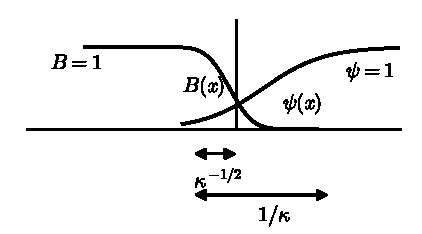
\includegraphics[width=6.3cm]{fig6.pdf}\\[0.3em]{\small 图 6}
\end{minipage}\par\nopagebreak

域内某处选取的. 这个解是
\begin{equation}
\psi=\tanh\bigl(\kappa x/\sqrt{2}\,\bigr).
\end{equation}
用这个函数（并且$A=0$）算出(46.12)式的积分，得：
\begin{equation}
\alpha_{ns}=\frac{H_{\mathrm{c}}^2\delta}{3\sqrt{2}\,\pi\kappa}
=\frac{H_{\mathrm{c}}^2}{8\pi}\,\frac{1.9\,\delta}{\kappa}.
\end{equation}
此值误差的产生是由于忽略了场减弱区域对积分的贡献. 为了估计这个区域的宽度$\delta_1$\footnote{应当强调，这个宽度不同于场从真空到超导体的穿透深度！从真空进到超导体时，在场的穿透区域内~$\psi\sim1$，当从~$n$相穿透时，场在小~$\psi$区域内减弱，}，我们指出：一方面，根据方程(46.9)，$\delta_1^{-2}\sim\psi^2$. 另一方面，公式(46.13)按其数量级来看，在$x\sim\delta_1$的区域边界上也仍然成立，因而$\psi\sim\kappa\delta_1$. 从这两个关系式我们求得$\delta_1\sim\kappa^{-1/2}$. 而这个区域对表面张力的贡献是$\sim H_{\mathrm{c}}^2\delta\kappa^{-1/2}$，即小于(46.14)式的值，它们的比仅为$\sim\kappa^{1/2}$［因此(46.14)式的精度是不高的］.

当参数$\kappa$增大时，表面张力系数经过零而变成负值. 这一点从下述事实便看得出来：当$\kappa$值足够大时，在任何情况下都存在不等式$\alpha_{ns}<0$. 事实上，在这个问题中函数$\psi(x)$变化的特征距离不可能小于$A(x)$变化的距离，因为$A$变化本身就导致$\psi$的变化；所以当$\kappa$较大时(46.12)式中积分号下的$\psi'^2/\kappa^2$项可以忽略不计，但由于$0<A'<1$（即在通常的单位中，$0<B<H_{\mathrm{c}}$），所以被积式是负的. 现在我们证明，当
\begin{equation}
\kappa=1/\sqrt{2}
\end{equation}
时，$\alpha_{ns}$将变为零.

为此，我们把$\alpha_{ns}$的表达式改写成如下形式：
\begin{equation}
\alpha_{ns}=\frac{H_{\mathrm{c}}^2\delta}{8\pi}\int_{-\infty}^{\infty}
\bigl[(A'-1)^2-\psi^4\bigr]\mathrm{d}x
\end{equation}
［此式得自(46.12)式的初积分，其中利用$\psi'^2$项的分部积分并随之代入(46.8)式的$\psi''$］. 假如被积式恒等于零，即如果
\begin{equation}
A'-1=-\psi^2,
\end{equation}
则积分显然变成零（此等式中取相反符号是不可能的，因为场$B=A'$随$x$的增大应当减小）. 由(46.17)和(46.9)两式消去$\psi$，求得方程
\begin{equation}
A''=A(1-A'),
\end{equation}
此方程的解（在$x=-\infty$时$A'=1$及$x=\infty$时$A=0$的边界条件下）确定了场的分布；因为有(46.17)式，于是$\psi$的边界条件(46.10)自然得到满足. 实际上不求解方程(46.18)便足以证明：当$\kappa^2=1/2$时，还未被利用的方程(46.8)或其初积分(46.11)，自然也被满足. 把(46.17)式代入(46.9)式，得到$\psi'=-A\psi/2$；这个$\psi'$值连同(46.17)中的$A'$事实上恒满足$\kappa^2=1/2$时的等式(46.11).

\begin{xiti}

对于参数$\kappa\ll1$的超导体，试求弱磁场中场对穿透深度的一级修正.

{\heiti 解：}我们选取超导体表面为$yz$面，其中$z$轴沿外场$\mathfrak{H}$的方向，并使$x$轴指向物体的内部，场和$\psi$在超导体中的分布由方程(46.8—46.9)确定，现在需要求解边界条件为
\begin{equation*}
\begin{array}{ll}
\psi'=0,\quad B=A'=\mathfrak{H},&\text{当 }x=0\text{ 时；}\\[0.2em]
\psi'=1,\quad A=0,&\text{当 }x=\infty\text{ 时}
\end{array}
\end{equation*}
的方程(46.8—46.9)［其中第一个边界条件就是条件(45.15)］. 我们来寻求如下形式的解：
\begin{equation*}
\psi=1+\psi_1(x),\qquad A=-\mathfrak{H}\mathrm{e}^{-x}+A_1(x),
\end{equation*}
式中$\psi_1$、$A_1$是$\kappa=0$时解的小修正，这个解对应于场按伦敦规律(44.13)的衰减. 对于修正量$\psi_1$，我们有方程
\begin{equation*}
\psi_1''=2\kappa^2\psi_1+\frac{1}{2}\kappa^2\mathfrak{H}^2\mathrm{e}^{-2x},
\end{equation*}
考虑到边界条件，因而
\begin{equation}\tag{1}
\psi_1=\frac{1}{8}\kappa^2\mathfrak{H}^2\mathrm{e}^{-2x}
-\frac{1}{4\sqrt{2}}\kappa\mathfrak{H}^2\mathrm{e}^{-\sqrt{2}\kappa x}
\end{equation}
现在我们写出关于$A_1$的方程：
\begin{equation*}
A_1''=A_1-2\mathfrak{H}\mathrm{e}^{-x}\psi_1,
\end{equation*}
对于式中的$\psi_1$，只需把$\kappa$一次方的(1)式第二项代入上式便可. 考虑到边界条件（$A_1'=0$，当$x=0$时）并且在此可以忽略系数中$\kappa$的高次项，我们求得
\begin{equation}\tag{2}
A_1=-\frac{1}{8}\mathfrak{H}^3\bigl[(1+\kappa\sqrt{2}\,)\mathrm{e}^{-x}
-\mathrm{e}^{-(1+\sqrt{2}\kappa)x}\bigr]
\end{equation}
因而求出了场对超导体深度方向的衰减规律的修正. 我们引入有效穿透深度$\delta_{\mathrm{eff}}$，根据定义，
\begin{equation*}
\mathfrak{H}\delta_{\mathrm{eff}}=\int_0^{\infty}B(x)\,\mathrm{d}x
=-A(0)=\mathfrak{H}-A_1(0).
\end{equation*}
恢复到通常的单位时，由(2)式可得：
\begin{equation*}
\delta_{\mathrm{eff}}=\delta\biggl[1+\frac{\kappa}{4\sqrt{2}}
\biggl(\frac{\mathfrak{H}}{H_{\mathrm{c}}}\biggr)^{\!2}\,\biggr].
\end{equation*}

\end{xiti}

\section{两类超导体}

表面张力$\alpha_{ns}$的符号，对超导体的性质有重要影响. 据此，把所有超导体分为两类：$\alpha_{ns}>0$的为第一类超导体，$\alpha_{ns}<0$的为第二类超导体. 因为$\alpha_{ns}$的符号决定于金兹堡-朗道参数$\kappa$的值，所以第一类对应于（在$T_{\mathrm{c}}$附近）$\kappa<1/\sqrt{2}$的值，而第二类对应于$\kappa>1/\sqrt{2}$的值\footnote{超导纯金属元素属于第一类超导体. 超导合金以及§43讲到的高温超导体属于第二类超导体. 关于在合金中~$\kappa>1/\sqrt{2}$的假设，是~Л.\,Д.\,朗道首先提出来的.}.

我们现在研究大尺度圆柱形超导体于纵向外磁场$\mathfrak{H}$中的情况. 如果属于第一类超导体，则当场增强并达到临界值$H_{\mathrm{c}}$时，它将经受第一级相变. 这时表面张力的作用（同一切第一级相变时一样），仅在于阻碍新相的首批晶核的形成，因而也就可能在场稍许超过$H_{\mathrm{c}}$时保持亚稳的$s$相.

如果属于第二类超导体，那么在场达到$H_{\mathrm{c}}$值之前，在热力学上就有利于产生$n$相的“掺杂”；并且体积能的增大将被所产生的晶核的负表面能抵消. 习惯上把能使这两种能量相消的场的下限值记为$H_{\mathrm{c}1}$，并称作下临界场. 同样，在大外场的情况下，从正常态金属开始，我们将得到称作上临界场的某个值$H_{\mathrm{c}2}>H_{\mathrm{c}}$，小于这个值，在热力学上有利于$s$相“掺杂”的产生，这又是依靠负边界能量的优势. 因此，在场的某个区间$H_{\mathrm{c}1}<\mathfrak{H}<H_{\mathrm{c}2}$内，可以说超导体处于混合态\footnote{勿把混合态同在样品和外磁场的一定配置下产生的第一类超导体的中间态混为一谈！}. 处于这种状态的超导体，其性质逐渐由$H_{\mathrm{c}1}$时的纯超导性变到$H_{\mathrm{c}2}$时的纯正常传导性；同时，发生磁场对超导体的逐渐穿透. $H_{\mathrm{c}}$值仅取决于$n$相和$s$相体积能之间的对比关系，而此值本身在这里没有什么值得重视的.

当然，两个临界场与温度有关，并当$T=T_{\mathrm{c}}$时它们都变为零. 由此可得出图7中所画的第二类超导体的相图（图中的虚曲线见下面）.

在金兹堡-朗道理论范围内，即使没有预先查明混合态结构的性质，也可以确定出上临界场. 这一点，通过下列问题便足以看得出来，当磁场稍小于$H_{\mathrm{c}2}$时，$s$相的晶核只能具有小的序参数$\psi$值（显然，当$\mathfrak{H}\to H_{\mathrm{c}2}$时，$\psi\to0$）. 因此这些晶核的状态可以用$\psi$的线性化的金兹堡-朗道方程来描述. 略去(45.12)式中的非线性项，我们得到方程：
\begin{equation}
\frac{1}{4m}\biggl(-\mathrm{i}\hbar\nabla-\frac{2e}{c}\bm{A}\biggr)^{\!2}\psi=|a|\psi,
\end{equation}
并且可以将$\bm{A}$理解为$\psi=0$时均匀场$\mathfrak{H}$的矢势，这时物体处在正常态，外场对它完全穿透.

但是(47.1)式，就其本身的形式来看，只不过是磁场中质量为$2m$、电荷为$2e$的粒子的薛定谔方程，其中$|a|$起着能级的作用；这两个问题的边界条件也是相同的：无穷远处，$\psi=0$. 我们知道（见第三卷§112），在均匀磁场中运动粒子能量的最小值是$E_0=\hbar\omega_H/2$，这里$\omega_H=2|e|\mathfrak{H}/2mc$（从此值起能谱是连续的）. 由两个问题之间具有的相似性得出：方程(47.1)所描述的$s$相的晶核，只有当
\begin{equation*}
|a|>\frac{|e|\hbar}{2mc}\mathfrak{H}
\end{equation*}
时才能存在. 因此临界场$H_{\mathrm{c}2}=2mc|a|/|e|\hbar$. 借助于表达式(45.9)、(45.17)和(45.18)，此公式可以写成
\begin{equation}
H_{\mathrm{c}2}=\sqrt{2}\,\kappa H_{\mathrm{c}}.
\end{equation}
（A.\,A.\,Абрикосов，1952）.

无穷远处的边界条件为$\psi=0$的方程(47.1)，它的解对应于在远离样品表面的深处形成$s$相晶核. 我们指出，表面的存在有助于晶核形成，因此甚至在$\mathfrak{H}>H_{\mathrm{c}2}$的情况下也能在薄表面层内产生晶核（D.\,Saint-James, P.\,G.\,De Gennes, 1963）.

描述物体表面（视为平面）附近$s$相晶核的方程(47.1)的解，在物体表面上应满足边界条件$\partial\psi/\partial x=0$（即$A_x=0$时的条件(45.15)］，这里$x$是沿表面法线

\par\nopagebreak\noindent\begin{minipage}{\linewidth}\centering
\begin{minipage}[t]{0.48\linewidth}\centering
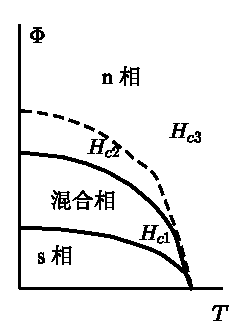
\includegraphics[width=4.9cm]{fig7.pdf}\\[0.3em]{\small 图 7}
\end{minipage}\hfill
\begin{minipage}[t]{0.48\linewidth}\centering
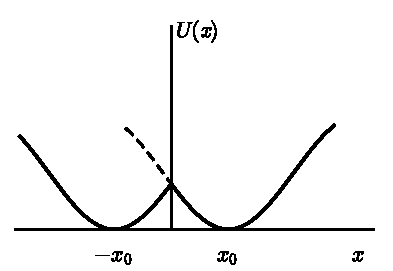
\includegraphics[width=5.2cm]{fig8.pdf}\\[0.3em]{\small 图 8}
\end{minipage}
\end{minipage}\par\nopagebreak

方向的坐标. 为了建立所要的量子力学类比，我们提醒一下：上边所利用的粒子在均匀磁场中的运动问题，同样等价于粒子一维抛物线势阱
\begin{equation*}
U=\frac{2m}{2}\omega_H^2(x-x_0)^2
\end{equation*}
中的运动问题，式中$x_0$是对应于“轨道中心”的常数（见第三卷§112）. 我们现在来研究一个双势阱，它是由对$x=0$平面（图8）对称分布的两条相同的抛物线势阱构成的. 在这种场中，对应于基态粒子的波函数$\psi(x)$没有零值而且是$x$的偶函数；这种函数自然满足$x=0$时$\psi'=0$的条件. 此时，双势阱中粒子的基态能级位于单势阱中的基态能级以下\footnote{这一点与~$x<0$的半空间内的势能低于单势阱（图8中的虚线）内的势能有关. 例如，参考第三卷§50的习题~3.}；转到关于晶核问题时，由此也可证明上述在表面附近容易形成晶核的论断.

对双势阱中的能级进行数值计算，得出的结果是：能级的最小值（决定于参数$x_0$）为$0.59E_0$. 重复导致公式(47.2)的讨论，我们得出产生$s$相表面晶核的场的上限值位于$H_{\mathrm{c}3}=H_{\mathrm{c}2}/0.59$附近，即
\begin{equation}
H_{\mathrm{c}3}=1.7\,H_{\mathrm{c}2}=2.4\,\kappa H_{\mathrm{c}}.
\end{equation}
因此，在$H_{\mathrm{c}2}$和$H_{\mathrm{c}3}$之间的场区域内将出现表面超导现象；这个区域的边界如图7中的虚线所示. 正常相表面附近超导层的厚度具有$\xi(T)$的数量级. 根据同样的量子力学类比不难得出上述估计，因为势阱中（在能级$E_0$上）粒子的波函数集中在$x\sim\hbar/\sqrt{mE_0}$区域内，把$E_0$换成$|a|$即可得出相应的晶核尺寸，根据(45.17)式，它与$\xi(T)$是相同的.

上边所说的都是关于第二类超导体的. 但是这样引入的临界场$H_{\mathrm{c}2}$和$H_{\mathrm{c}3}$，对第一类超导体也具有确定的物理意义.

如果$\kappa$位于$1/\sqrt{2}=0.71>\kappa>0.59/\sqrt{2}=0.42$区域内，则$H_{\mathrm{c}2}<H_{\mathrm{c}}$，但$H_{\mathrm{c}3}>H_{\mathrm{c}}$. 虽然在这种情况下并不产生混合相，但在$H_{\mathrm{c}}$和$H_{\mathrm{c}3}$之间的场区间内却存在表面超导性.

最后，按得出结论的意义来看，当$\kappa$为任何值时，(47.2)式的$H_{\mathrm{c}2}$的值都将确定场的上限，而在这个场中可以形成$\psi$值为任意小的$s$相晶核. 因此，在场$\mathfrak{H}<H_{\mathrm{c}2}$中的第一类超导体内（其中$H_{\mathrm{c}2}<H_{\mathrm{c}}$），在热力学上不利的正常相是完全不稳定的. 但在$H_{\mathrm{c}2}<\mathfrak{H}<H_{\mathrm{c}}$区间内，正常相可以作为亚稳态而存在：在这个场区间内，从$n$相到$s$相的第一级相变，只能借助于$\psi$为有限值的$s$相晶核的产生，但晶核的产生受到两相界面上的正表面张力的阻碍（В.\,Л.\,金兹堡，1956）.

\begin{xiti}

试求半径为$R\ll\delta$的超导小球的临界场（В.\,Л.\,金兹堡，1958）.

{\heiti 解：}同薄膜中的情况一样——（见§45的习题），此时发生超导性的破坏，是由于第二级相变. 我们所求的小球的临界场是这样的场值：低于它，$n$相便失去稳定性而形成$s$相晶核像正文中所说的一样，这归结于寻求薛定谔方程(47.1)的最小本征值. 在$R\ll\delta$的条件下，这个本征值可以借助于关于外场的微扰论求出，此时无微扰波函数$\psi=$常数（晶核占据整个小球体积）. 于是本征值单纯就由微扰算符$(2e\bm{A}/c)^2/4m$的平均值来确定［当$\psi=$常数时，算符$(\mathrm{i}e\hbar/mc)(\bm{A}\cdot\nabla)$的平均值等于零］. 这时，均匀场的矢势应当取$\bm{A}=\mathfrak{H}\times\bm{r}/2$的形式；正是在这种规范下，$\psi=$常数的解在小球表面上满足边界条件(45.15)，这个条件归结于要求$\bm{n}\cdot\bm{A}=0$. 进行平均，得到
\begin{equation*}
E_0=\frac{e^2}{4mc^2}\,\frac{2}{3}\,\mathfrak{H}^2\,\overline{r^2}
=\frac{e^2\mathfrak{H}^2R^2}{10mc^2}.
\end{equation*}
同正文一样，利用条件$E_0=|a|$即可求出临界场，得出的结果为：
\begin{equation*}
H_{\mathrm{c}}^{(\text{球})}=\sqrt{20}\,H_{\mathrm{c}}\delta/R.
\end{equation*}
之所以允许利用微扰论，为如下事实所证实. 已得出的$E_0$值（当$\mathfrak{H}=H_{\mathrm{c}}^{(\text{球})}$时），在$R\ll\delta$的条件下，确实小于随后的本征值，此值对应于小球体积中已经变化的波函数，并且有$\hbar^2/mR^2$的数量级.

\end{xiti}

\section{混合态的结构}

像上一节一样，我们重新研究圆柱形第二类超导体样品于纵向磁场$\mathfrak{H}$中的情形. 我们现在阐明处在少许超过下临界场$H_{\mathrm{c}1}$的磁场中物体的混合态结构\footnote{这一节里（以及本节的习题中）所讲述的结果，是属于~А.\,А.\,Абрикосов 的工作（1957）.}.

在这种情况下，基本超导相中掺入一些正常相的晶核. 为了获得最大的热力学的有利性，这些晶核（在负表面张力的情况下！）应具有尽可能大的表面. 因此自然是这样的结构：其中$n$相的晶核是一些平行于场方向的线. 在这些线（称作涡线）的附近，既聚集有穿透物体的磁场，也有围绕涡线的环形超导电流.

外场越接近$H_{\mathrm{c}1}$，物体中这些涡线越少，而各线之间的距离也越大. 当距离足够大时，§44中最后所叙述的见解便适用于各单独的涡线. 根据这个见解，聚集在涡线附近的总磁通量必定是基本磁通量量子$\phi_0=\pi\hbar c/|e|$的整数倍；下边我们将会看到，涡线具有最小可能的通量（只有$\phi_0$）在热力学上是有利的. 正是$\phi_0$的有限性给正常相晶核继续的分裂规定了极限.

当外场从小增大并达到$H_{\mathrm{c}1}$值时，在圆柱体内将出现一条涡线. 我们现在写出决定这个时机的热力学条件. 这时，首先并不去注意涡线本身的结构，而只考虑与涡线有关的某一（正的！）能量；我们把属于单位长度涡线的这个能量记为$\varepsilon$（以后将算出这个能量值）.

显然，圆柱形物体在纵向外场中，磁感应强度$\bm{B}$也处处沿圆柱体的轴线方向. §46中引入的宏观场强$\bm{H}=\bm{B}-4\pi\bm{M}$也是如此. 于是由方程$\nabla\times\bm{H}=0$得出：$\bm{H}$沿圆柱体截面（因此整个体积）处处不变；由于$\bm{H}$的切向分量的连续性边界条件，这个恒定值与外场相等：$\bm{H}=\mathfrak{H}$. 所以，我们需要研究在给定物体的体积、温度和场强$\bm{H}$的情况下物体的热力学平衡. 这种平衡的条件是：热力学势$\tilde{F}$对指定的变量取极小值（见第八卷§31）. 令$\tilde{F}_{\mathrm{s}}$是超导圆柱体的热力学势（因为在超导相中$\bm{B}=0$，所以$\tilde{F}_{\mathrm{s}}$与自由能$F_{\mathrm{s}}$相等）. 这时，具有一条涡线的圆柱体的热力学势为
\begin{equation*}
\tilde{F}=\tilde{F}_{\mathrm{s}}+L\varepsilon-\int\frac{\bm{H}\cdot\bm{B}}{4\pi}\,\mathrm{d}V
=F_{\mathrm{s}}+L\varepsilon-\frac{\mathfrak{H}}{4\pi}\int B\,\mathrm{d}V.
\end{equation*}
$L\varepsilon$项是涡线的自由能（$L$是线的长度，它与圆柱体长度相同），最后一项是热力学势$\tilde{F}$与自由能$F$的差别. 因为物体中的磁感应强度$\bm{B}$只集聚在涡线附近，所以$\int B\,\mathrm{d}V=L\phi_0$，这里$\phi_0$是通过涡线截面的磁感应通量. 因此
\begin{equation}
\tilde{F}=\tilde{F}_{\mathrm{s}}+L\varepsilon-\frac{L\phi_0\mathfrak{H}}{4\pi}.
\end{equation}
当$\tilde{F}_{\mathrm{s}}$的附加量为负值时，产生涡线在热力学上有利. 若使附加量等于零，我们便求得外场的临界值：
\begin{equation}
H_{\mathrm{c}1}=4\pi\varepsilon/\phi_0.
\end{equation}

我们现在来研究单个的涡线结构. 我们只限于讨论当
\begin{equation}
\kappa\gg1
\end{equation}
即$\delta\gg\xi$时的重要情况. $\xi$的长度确定涡线“蕊”半径的数量级，$|\psi|^2$在这个长度内从零（对应于涡线轴线上的正常态）变到对应于基本$s$相的有限值；在距涡线轴线的大距离$r$上，$|\psi|^2$保持恒定\footnote{在这一节里，字母~$r$表示圆柱坐标，即到轴线的距离.}. 而磁感应强度$B(\bm{r})$变化得相当缓慢，只在$r\sim\delta\gg\xi$的距离上才衰减. 换言之，全部磁通量基本上穿过涡线蕊以外的区域，这里$|\psi|^2=$常数（图9）.

\par\nopagebreak\noindent\begin{minipage}{\linewidth}\centering
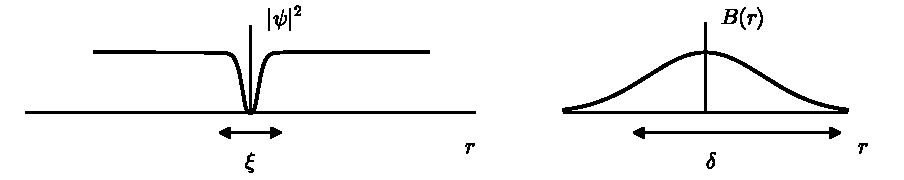
\includegraphics[width=10.2cm]{fig9.pdf}\\[0.3em]{\small 图 9}
\end{minipage}\par\nopagebreak

对于上述情况，可以运用伦敦方程（应注意，方程的适用性与温度向$T_{\mathrm{c}}$的趋近无关）求出场的分布. 在这里为了赋予方程以所需要的形式，首先改写联系波函数相位与超导电流密度的公式(44.7)：
\begin{equation}
\bm{A}+\delta^2\,\nabla\times\bm{B}=\frac{\phi_0}{2\pi}\,\nabla\bm{\Phi},
\end{equation}
此式中引入了穿透深度$\delta$，并把$\bm{j}$用磁感应强度表示出来$\bm{j}=c\,\nabla\times\bm{B}/4\pi$. 这里伦敦近似相当于假设$\delta=$常数. 我们将等式(48.4)沿闭合回路$C$求积分，该回路围绕涡线并在离涡线轴线为$r\gg\xi$的距离上通过. 根据斯托克斯定理，将$\bm{A}$的积分变换成对回路所围的面积的积分，我们得到：
\begin{equation}
\int\bm{B}\cdot\mathrm{d}\bm{f}+\delta^2\oint\nabla\times\bm{B}\cdot\mathrm{d}\bm{l}=\phi_0,
\end{equation}
将第二个积分也作同样的变换，可写成
\begin{equation}
\int\bigl[\bm{B}+\delta^2\,\nabla\times(\nabla\times\bm{B})\bigr]\cdot\mathrm{d}\bm{f}=\phi_0
\end{equation}
等式右边写出对应于相位只增加一个$2\pi$的（不等于零的）最小可能值. 如果回路$C$在离涡线为$r\gg\delta$的距离上通过，此处场和电流已经可以认为是不存在的，则(48.5)式中的第二个积分便可以忽略，因而我们看到，$\phi_0$与聚集在单个涡线周围的总磁感应通量是相同的. 但涡线的轴线本身是一条奇异线，环绕奇异线时将改变波函数的相位.

因为对于任一回路$C$（满足上面指出的条件）等式(48.6)都应得到满足，所以根据这个等式应当有：
\begin{equation}
\bm{B}+\delta^2\,\nabla\times(\nabla\times\bm{B})
=\bm{B}-\delta^2\Delta\bm{B}=\phi_0\delta(\bm{r}),
\end{equation}
式中$\bm{r}$是涡线横截平面内的二维径矢. 在这个方程的右边记入$\delta$函数的形式，表示这里$\sim\xi$的距离都看作是零. 在整个空间里，除$\bm{r}=0$的线以外，(48.7)式与伦敦方程(44.11)是一致的，但对于描述涡线，需要$\bm{r}=0$时具有奇异性的解.

在$\delta\gg r\gg\xi$的区域内，距离轴线为$r$处的场的分布可以由(48.5)式直接求出. 我们选取这个区域中的半径为$r$的圆周作为回路$C$. 通过这个回路的磁感应通量［(48.5)式左边的第一项］仅仅是全部磁通量的一小部分，即它的$\sim(r/\delta)^2$部分；因而我们把它略去不计. 在第二项中$\mathrm{d}\bm{l}$是圆周的长度元，因为矢量$\bm{B}$的方向沿着$z$轴（以涡线的轴线为柱坐标系的轴）因而它只与$r$有关，所以
\begin{equation*}
\bm{l}\cdot(\nabla\times\bm{B})=(\bm{l}\times\nabla)\cdot\bm{B}
=-\frac{\partial B_z}{\partial r}=-\frac{\mathrm{d}B}{\mathrm{d}r},
\end{equation*}
（$\bm{l}$是与圆周相切的单位矢量）. 因此我们获得方程：
\begin{equation}
\bm{l}\cdot(\nabla\times\bm{B})=-\frac{\mathrm{d}B}{\mathrm{d}r}
=\frac{\phi_0}{2\pi r\delta^2}.
\end{equation}
由此
\begin{equation}
B(r)=\frac{\phi_0}{2\pi\delta^2}\ln\frac{\delta}{r},\qquad \xi\ll r\ll\delta.
\end{equation}
由于这种关系具有对数性质，积分上限（在此处应当是$B\approx0$）可以规定与所研究的距离$r$的上界相一致.

为了将求得的分布延拓在$r\gtrsim\delta$的区域，我们运用对一切$r\gg\xi$都适用的方程(48.7). 把拉普拉斯算符在柱坐标中展开，［考虑到$\bm{B}=\bm{B}_z(r)$］，我们可将方程（当$r\neq0$时）重写成如下形式：
\begin{equation*}
B''+\frac{1}{r}B'+\delta^{-2}B=0,
\end{equation*}
当$r\to\infty$时这个方程具有递减的解：
\begin{equation*}
B(r)=\text{常数}\times K_0(r/\delta).
\end{equation*}
式中$K_0$是马克多纳（Macdonald）函数［即虚宗量的汉克尔（Hankel）函数］. 常系数通过与解(48.9)的“接合”来确定：这时需利用熟知的$z\ll1$时的极限表达式$K_0(z)\approx\ln(2/z\gamma)$，而$\gamma=\mathrm{e}^{\mathrm{c}}=1.78$. 于是最终有
\begin{equation}
B(r)=\frac{\phi_0}{2\pi\delta^2}K_0\biggl(\frac{r}{\delta}\biggr),\qquad r\gg\xi.
\end{equation}
特别是，借助熟悉的$z\to\infty$时的渐近表达式$K_0(z)\approx(\pi/2z)^{1/2}\mathrm{e}^{-z}$，便求得远离涡线轴线的衰减规律：
\begin{equation}
B(r)=\frac{\phi_0}{(8\pi r\delta^3)^{1/2}}\,\mathrm{e}^{-r/\delta}.
\end{equation}
我们注意到超导体中和液氦中（§29）涡线的性质很相似. 在这两种情况都谈及了奇异线，绕这些奇异线环绕时将改变凝聚体波函数的相位. 在液氦中环绕涡线超流运动的环形轨道，相当于超导体中的环形电流；超流运动的速率$v_{\mathrm{s}}$按$1/r$的规律减小，超导电流密度也按同样规律减小，如：
\begin{equation}
j=\frac{c}{4\pi}\,|\nabla\times\bm{B}|=\frac{c\phi_0}{8\pi^2\delta^2 r}.
\end{equation}
这种吻合是完全自然的，因为两种情况这些规律都是存在奇异线的直接结果. 不过，在液氦中上述$v_{\mathrm{s}}(r)$的依赖关系可延伸到任何距离，而在超导体中当$r\gg\delta$时$j(r)$便按指数规律减小. 这一差别与电子液体的带电性有关，因为带电粒子运动会产生磁场，同样地，这种运动也屏蔽磁场（如果粒子的电荷$e$趋于零，则穿透深度$\delta\to\infty$）.

现在可以计算涡线的自由能. 蕊外（$r\gg\xi$）的空间区域对自由能的贡献，由对这个区域所取的积分给出：
\begin{equation}
F_{\text{蕊}}=\frac{1}{8\pi}\int\bm{B}^2\,\mathrm{d}V
+\frac{\delta^2}{8\pi}\int(\nabla\times\bm{B})^2\,\mathrm{d}V.
\end{equation}
事实上，将这个表达式对$\bm{B}$取变分（当给定温度，即给定$\delta$时），我们便直接得到$\bm{r}\neq0$的伦敦方程(48.7)\footnote{(48.13)式中的第二项用电流~$\bm j$表达时取如下形式：
\begin{equation*}
2\pi c^2\delta^2\int\bm j^2\,\mathrm dV=\int\frac{\rho_{\mathrm s}\bm v_{\mathrm s}^2}{2}\,\mathrm dV.
\end{equation*}
在第二个表达式中再作代换：$\delta^2=mc^2/(4\pi e^2n_{\mathrm s})$，并按~$\bm j=e\rho_{\mathrm s}\bm v_{\mathrm s}/m$引入超流分量的密度和速度.（见165页的注解），我们看到，这一项可看作是超导电子的动能.}. (48.13)式中的第二个积分，在$\delta\gg r\gg\xi$区域的两个边界上呈对数发散，它远大于第一个积分. 把(48.8)式中的$|\nabla\times\bm{B}|$代入上式，我们得到单位长度涡线的能量：
\begin{equation}
\varepsilon=\biggl(\frac{\phi_0}{4\pi\delta}\biggr)^{\!2}\ln\frac{\delta}{\xi}.
\end{equation}
此式具有对数准确度，即不仅要求$\delta/\xi\gg1$，而且也要求$\ln(\delta/\xi)\gg1$；正是由于有这种准确度，才可以忽略涡线蕊对$\varepsilon$的贡献.

特别是，由(48.14)式的结果能够证明上边得出的论断，即产生具有最小磁通量值的涡线在热力学上是有利的. 事实上，因为涡线的自由能与同涡线有关的磁通量的平方成比例，所以对于磁通量为$n\phi_0$的涡线来说，在能量中将出现一个因子$n^2$；再把这样的涡线分解成$n$条磁通量为$\phi_0$的涡线时，将使能量赢余$n$倍.

将(48.14)式代入(48.2)式，我们求得下临界场
\begin{equation}
H_{\mathrm{c}1}=\frac{\phi_0}{4\pi\delta^2}\ln\frac{\delta}{\xi},
\end{equation}
当$T\to T_{\mathrm{c}}$时，考虑到(45.19)式，上式也可以写成
\begin{equation}
H_{\mathrm{c}1}=H_{\mathrm{c}}\,\frac{\ln\kappa}{\sqrt{2}\,\kappa}\ \footnotemark.
\end{equation}
\footnotetext{因为这个函数是根据假设~$\ln\kappa\gg1$导出的，当~$\kappa\sim1$时绝不能用它！其中，当~$\kappa=1/\sqrt{2}$时，场~$H_{\mathrm{c}1}$（和~$H_{\mathrm{c}2}$一样）自然应与~$H_{\mathrm{c}}$相等.}
随着外场的增强，涡线数量增多，因而磁场对超导体的穿透增强了. 在计算涡线之间的相互作用时，热力学平衡对应于涡线的一定的有序分布，后者构成了二维格子（在圆柱体的截面内）\footnote{看来，涡线在格点形成等边三角形时格子最为有利.}. 在任何涡线数密度下，每一条涡线的轴线仍旧是一直线，环绕这条轴线波函数的相位将改变$2\pi$. 磁感应强度对圆柱体截面的平均值
\begin{equation}
\overline{B}=\nu\phi_0,
\end{equation}
式中$\nu$是通过单位截面积的涡线数. 事实上，如果把关系式(48.4)沿样品整个截面的回路求积分，那么便得出方程(48.5)，其右边为$S\nu\phi_0$（$S$是截面积）；方程左边的第一个积分是总磁感应通量$S\overline{B}$，而第二个积分是边缘效应，它小于第一个积分，它们的比值为$\sim\delta/R$（$R$是截面的线度），因此它可以忽略不计；当然，这里重要的是：在距离为$\sim\delta$处环绕涡线的磁场将发生衰减.

只要各涡线之间的距离$d$大于关联半径$\xi$，就可以断言：涡线磁场是单纯叠加的. 事实上，当$d\gg\xi$时，仍然可以划出包围任何数目涡线的回路，并使它处处在远离涡线蕊（距离$\gg\xi$）的地方通过. 在这种回路上满足伦敦近似条件（$\delta$不变），因此我们又重新获得稍异于(48.7)式的方程，其中右边的$\delta$函数换成宗量为到每条涡线距离的$\delta$函数之和. 由于这个方程是线性的，因而便得出上述论断.

当外场接近于$H_{\mathrm{c}2}$时，涡线间的距离就可以同$\xi$相比较了. 这一点，也可以从临界场表达式(47.2)本身清楚地看出来，如果借助(45.9)及(45.16—45.18)式，可将(47.2)式写成
\begin{equation}
H_{\mathrm{c}2}=\phi_0/2\pi\xi^2,
\end{equation}
此式对应于集中在面积为$\sim\xi^2$上的通量$\phi_0$.

当$\mathfrak{H}=H_{\mathrm{c}2}$时，发生第二级相变，超导性消失了. 就这种相变的一般理论的实质来说，可以断言：作为外场函数的序参数$\psi$将按$|\psi|^2\propto H_{\mathrm{c}2}-\mathfrak{H}$的规律变为零. 另一方面，物质的磁化强度$\bm{M}=(\bm{B}-\bm{H})/4\pi$自身（系与$\psi$的相位选取无关的量）在这个区域内与$|\psi|^2$成比例. 考虑到$\mathfrak{H}=H_{\mathrm{c}2}$时必有$B=H_{\mathrm{c}2}$，因此我们得到超导体中的磁感应强度$B$在相变点附近依赖于外场的如下线性规律：
\begin{equation}
B-H_{\mathrm{c}2}\propto\mathfrak{H}-H_{\mathrm{c}2}.
\end{equation}

\begin{xiti}

1. 试计算彼此相距$d\gg\xi$的两条涡线的相互作用能.

{\heiti 解：}我们将两条涡线系统的自由能表达式(48.13)变换一下形式：其中只在每一条单独涡线附近进行积分. 为此，利用方程(48.7)，我们写出：
\begin{equation*}
\bm{B}^2+\delta^2(\nabla\times\bm{B})^2
=\delta^2\bigl\{-\bm{B}\cdot\nabla\times(\nabla\times\bm{B})+(\nabla\times\bm{B})^2\bigr\}
=\delta^2\,\nabla\cdot(\bm{B}\times\nabla\times\bm{B})
\end{equation*}
把体积积分变换成如下积分：
\begin{equation}\tag{1}
F_{\text{蕊}}=\frac{\delta^2}{8\pi}\int_{f_1+f_2}
\bigl[\bm{B}\times(\nabla\times\bm{B})\bigr]\cdot\mathrm{d}\bm{f},
\end{equation}
此式是沿包围涡线蕊的圆柱形表面$f_1$和$f_2$（其小半径为$r_0$；$\xi\ll r_0\ll\delta$）取的积分. 当$d\gg\xi$时，涡线磁场是可加的，即$\bm{B}=\bm{B}_1+\bm{B}_2$. 涡线的相互作用能，由积分(1)中同时与$\bm{B}_1$和$\bm{B}_2$有关的部分给出：
\begin{equation*}
L\varepsilon_{12}=\frac{\delta^2}{8\pi}
\biggl\{\int(\bm{B}_2\times\nabla\times\bm{B}_1)\cdot\mathrm{d}\bm{f}_1
+\int(\bm{B}_1\times\nabla\times\bm{B}_2)\cdot\mathrm{d}\bm{f}_2\biggr\}
\end{equation*}
（当$r_0\to0$时，$\int(\bm{B}_2\times\nabla\times\bm{B}_1)\cdot\mathrm{d}\bm{f}_2$形状的积分趋于零）. 利用(48.8)和(48.10)式而得出：
\begin{equation*}
\varepsilon_{12}=2\,\frac{\delta^2}{8\pi}\,2\pi r_0\,\frac{\phi_0}{2\pi r_0\delta^2}\,B(d)
=\frac{\phi_0^2}{8\pi^2\delta^2}\,K_0\biggl(\frac{d}{\delta}\biggr),
\end{equation*}
特别是，在距离$d\gg\xi$处：
\begin{equation}\tag{2}
\varepsilon_{12}=\frac{\phi_0^2}{2^{7/2}\pi^{3/2}\delta^2}
\biggl(\frac{\delta}{d}\biggr)^{\!1/2}\mathrm{e}^{-d/\delta}.
\end{equation}

2. 如圆柱体样品截面的平均磁感应强度为$\overline{B}$，试求$\overline{B}$对混合态中外场$\mathfrak{H}$的依赖关系. 处于这种状态时，各涡线都分布在彼此相距$d\gg\delta$的地方，这时，在样品的截面内构成等边三角形格子.

{\heiti 解：}等边三角形的面积等于$\sqrt{3}\,d^2/4$（$d$是边长），而涡线数等于格子中三角形数的一半（$N$个三角形有$3N$个格点，但格子中每一格点是属于六个最相邻的三角形的），因此$\nu=2/\sqrt{3}\,d^2$.

处于混合态的物体，其单位体积的热力学势为
\begin{equation*}
\tilde{f}=\tilde{f}_{\mathrm{s}}-\frac{\phi_0}{4\pi}\,\nu(-H_{\mathrm{c}1}+\mathfrak{H})
+\frac{1}{2}\sum_{i,k}\varepsilon_{ik}.
\end{equation*}
式中第二项对应于表达式(48.1)［其中$H_{\mathrm{c}1}$由(48.2)式给出］；在第三项中，$\varepsilon_{12}$是两条涡线的相互作用能，并对穿过单位面积的全部涡线进行求和. 因为当$d\gg\delta$时$\varepsilon_{12}$按指数规律减小，所以求和式中只考虑相邻成对的那些线就足够了. 在三角形格子中，每条涡线有6个最相邻的线，因此
\begin{equation*}
\frac{1}{2}\sum_{i,k}\varepsilon_{ik}=\frac{6}{2}\sum_i\varepsilon_{i1}=3\nu\,\varepsilon_{12}(d).
\end{equation*}
把上题公式(2)中的$\varepsilon_{12}$代入上式，得：
\begin{equation*}
\tilde{f}=\tilde{f}_{\mathrm{s}}+\frac{\phi_0}{2\sqrt{3}\,\pi\delta^2}
\biggl[-\frac{\mathfrak{H}-H_{\mathrm{c}1}}{a^2}
+\frac{3\phi_0}{2\sqrt{2\pi}\,\delta^2}\,\frac{l^{-a}}{a^{5/2}}\biggr],
\end{equation*}
式中$a=d/\delta$，$a$与$\mathfrak{H}$的依赖关系决定于函数$\tilde{f}(a)$取极小值的条件；由此得出：
\begin{equation}\tag{3}
\mathfrak{H}-H_{\mathrm{c}1}=\frac{3\phi_0}{4\sqrt{2\pi}\,\delta^2}\,\sqrt{a}\,\mathrm{e}^{-a}.
\end{equation}
（这里省略了$1/a\ll1$的更高次项）. 这个方程连同等式$\overline{B}=\nu\phi_0$，即
\begin{equation*}
a=\bigl(2\phi_0/\sqrt{3}\,\delta^2\overline{B}\bigr)^{1/2}.
\end{equation*}
可确定待求的依赖关系$\overline{B}(\mathfrak{H})$. 应注意，当$\mathfrak{H}\to H_{\mathrm{c}1}$时，微商$\mathrm{d}\overline{B}/\mathrm{d}\mathfrak{H}$按
\begin{equation*}
\frac{\mathrm{d}\overline{B}}{\mathrm{d}\mathfrak{H}}
\propto\frac{1}{\mathfrak{H}-H_{\mathrm{c}1}}\ln^{-3}\frac{1}{\mathfrak{H}-H_{\mathrm{c}1}}.
\end{equation*}
这一规律趋于无穷大.

\end{xiti}

\section{高于相变点的抗磁磁化率}

在§45末曾经指出，序参数$\psi$的涨落在$T_{\mathrm{c}}$附近的温区变大，而超导体的这个温区是非常狭窄的. 在该区域以外，热力学量涨落的修正，一般地说是很小的. 但是，对于高于相变点的金属的磁化率来说，这些修正还是很重要的：由于涨落，即使有相当少数的超导电子出现，便能对磁化率有贡献. 这种贡献大于远离相变点的正常金属所提供的，后者的磁化率通常是很小的\footnote{这个效应是~В.\,В.\,Шмит（V.\,V.\,Shmidt）（1966）指出的.}.

现在我们研究处在弱外磁场（$\mathfrak{H}\ll H_{\mathrm{c}}$）中温度超过$T_{\mathrm{c}}$点但在该点附近的金属. 这里，序参数的平衡值$\psi=0$，为了算出$\psi$的涨落需要运用金兹堡-朗道理论中的自由能. 这时，在表达式(45.10)中（注意：涨落很小）只保留$\psi$的平方项，而略去$|\psi|^4$的项，并把$\bm{A}$理解为均匀场$\mathfrak{H}$的矢势，与$\psi$的涨落相关的磁感应强度$\bm{B}$的涨落是$\psi$的平方项（由于电流密度$\bm{j}$取平方）. 因此，忽略$\bm{B}$的涨落时，在$B^2/8\pi$项中就可以将$B$理解为磁感应强度的（热力学）平均值. 所以在有涨落的情况下，金属总自由能的变化由如下的表达式——$\psi$的泛函给出\footnote{为避免误解起见，我们强调指出：对于超导体，磁场并不是在第五卷§144中所引入的那种意义的“外场”~$h$. 后者，本来应当以~$-h(\psi+\psi^{*})$项的形式包含在自由能之中，但在目前的情况下显然是不可能的，因为这样的项对于~$\psi$的相位的选取不是不变的.}：
\begin{equation}
\Delta F[\psi]=\int\biggl\{\frac{1}{4m}
\biggl|\biggl(-\mathrm{i}\hbar\nabla-\frac{2e}{c}\bm{A}\biggr)\psi\biggr|^2
+a|\psi|^2\biggr\}\mathrm{d}V
\end{equation}
为计算对自由能的涨落的贡献$\Delta F$，需要把泛函(49.1)视为“等效哈密顿量”，由此根据公式
\begin{equation}
\exp\biggl(-\frac{\Delta F}{T}\biggr)
=\int\exp\biggl(-\frac{\Delta F[\psi]}{T}\biggr)D\psi
\end{equation}
可求出$\Delta F$，这里是对$\psi(\bm{r})$的全部分布求泛函积分（见第五卷§147）. 这一积分，实际上可以这样实现：将$\psi$展成某一完备的本征函数系，并对这个展开式的无穷多个系数求积分. 在无外场的均匀系统的情况下，可以简单地展成平面波（例如，参看第五卷§147中的习题）.

但在目前的情况下，应按哈密顿量(49.1)的“薛定谔方程”
\begin{equation}
\frac{1}{4m}\biggl(-\mathrm{i}\hbar\nabla-\frac{2e}{c}\bm{A}\biggr)^{\!2}\psi=E\psi
\end{equation}
的本征函数进行展开. 在§47中曾经指出，这个方程与均匀磁场中粒子（质量为$2m$，电荷为$2e$）运动薛定谔方程在形式上是一致的. 方程的本征函数用一个离散的（$n$）和两个连续的（$p_x$、$p_z$）量子数编号，而本征值只与$n$和$p_z$（$z$轴沿$\mathfrak{H}$的方向）有关，并由如下公式给出：
\begin{equation}
E\biggl(n+\frac{1}{2},p_z\biggr)=\biggl(n+\frac{1}{2}\biggr)\frac{|e|\hbar}{mc}\,\mathfrak{H}
+\frac{p_z^2}{4m},
\end{equation}
不同本征函数（具有给定的$n$、$\mathrm{d}p_z$区间内的$p_z$和所有可能的$p_x$值）的数目为
\begin{equation*}
V\,\frac{2|e|\mathfrak{H}}{(2\pi\hbar)^2c}\,\mathrm{d}p_z
\end{equation*}
（见第三卷§112）.

为简便起见，我们把量子数$n$、$p_x$、$p_z$的集合用一个记号$q$来表示，因而我们将函数$\psi(\bm{r})$的展开式写成
\begin{equation}
\psi=\sum_q c_q\psi_q(\bm{r}),
\end{equation}
式中$c_q=c_q'+\mathrm{i}c_q''$是任意的复系数，而本征函数满足归一化条件：$\int|\psi|^2\mathrm{d}V=1$（这里是按金属体积求积分）.

将展开式(49.5)代入(49.1)式，首先可把对体积求积分变为对$q$求和. 事实上，将第一项进行分部积分，便得出(49.1)式的如下形式：
\begin{equation*}
\Delta F[\psi]=\int\biggl\{\psi^*\,\frac{1}{4m}
\biggl(-\mathrm{i}\hbar\nabla-\frac{2e}{c}\bm{A}\biggr)^{\!2}\psi+\psi^*a\psi\biggr\}\mathrm{d}V
\end{equation*}
将(49.5)式代入上式，并考虑到每一个函数$\psi_q$都满足方程(49.3)（其中$E=E_q$），以及不同$q$的本征函数是相互正交的，我们便得：
\begin{equation}
\Delta F[\psi]=\sum_q|c_q|^2(E_q+a).
\end{equation}
(49.2)式中的泛函积分是指对所有$\mathrm{d}c_q'\mathrm{d}c_q''$求积分. 作(49.6)式的代换之后，按所有这些变量分开积分，因而得出：
\begin{equation}
\begin{gathered}
\exp\biggl(-\frac{\Delta F}{T}\biggr)=\prod_q\frac{\pi T}{E_q+a},\\
\text{或}\qquad
\Delta F=-T\sum_q\ln\frac{\pi T}{E_q+a}.
\end{gathered}
\end{equation}
用量子数$n$和$p_z$的术语，此表达式可写成
\begin{equation}
\Delta F=-V\,\frac{2|e|T\mathfrak{H}}{(2\pi\hbar)^2c}\sum_n
\int_{-\infty}^{\infty}\ln\frac{\pi T}{E(p_z,n+1/2)+a}\,\mathrm{d}p_z.
\end{equation}
这个求和式当$E$很大时是发散的，但这种发散实际上是虚假的，并只与这一情况有关：原来的公式(49.1)仅在函数$\psi(\bm{r})$缓慢改变（即在$\sim\xi_0$的距离上$\psi$的变化很小）时才适用. 用本征值$E_q$的术语，其意思是只允许$E_q\ll\hbar^2/m\xi_0^2$. 在满足所提条件的某大$N$处截断对$n$的求和，我们利用泊松公式
\begin{equation*}
\sum_{n=0}^{N}f\biggl(n+\frac{1}{2}\biggr)\approx
\int_0^N f(x)\,\mathrm{d}x-\frac{1}{24}f'(x)\Big|_0^N
\end{equation*}
［见第五卷(59.10)式］于(49.8)式时，不难理解：这个公式第一项的积分给出与$\mathfrak{H}$无关的对自由能的贡献；这一项对磁化率的计算并不需要，因而我们把它略去. 而在第二项中现在可以取$N\to\infty$（因此答案中去掉了截断参数）\footnote{在系数中取~$T\approx T_{\mathrm{c}}$. 当~$T$在~$T_{\mathrm{c}}$附近时，这个积分中的几个重要的值~$p_{\mathrm z}\sim\sqrt{ma}\sim\hbar/\xi(T)\ll\hbar/\xi_0$，即它们都满足所提出的条件.}：
\begin{equation*}
\Delta F=V\,\frac{e^2T_{\mathrm{c}}\mathfrak{H}^2}{48\pi^2\hbar mc^2}
\int_{-\infty}^{\infty}\frac{\mathrm{d}p_z}{a+p_z^2/4m},
\end{equation*}
最终求积分后，
\begin{equation}
\Delta F=V\,\frac{e^2T_{\mathrm{c}}\mathfrak{H}^2}{24\pi\hbar c^2\sqrt{ma}},
\end{equation}
从而磁化率
\begin{equation}
\chi=-\frac{1}{V}\frac{\partial^2\Delta F}{\partial\mathfrak{H}^2}
=-\frac{e^2T_{\mathrm{c}}}{12\pi\hbar c^2\,(ma)^{1/2}(T-T_{\mathrm{c}})^{1/2}}.
\end{equation}
（H.\,Schmidt, 1968; A.\,Schmid, 1969）. 我们看到，当温度接近于相变点时磁化率将随$(T-T_{\mathrm{c}})^{-1/2}$而增大. 在这个区域内，(49.10)式是对正常金属磁化率的主要贡献.

\begin{xiti}

1. 一薄膜（厚度$d\ll\xi(T)$）处于垂直于其平面的弱磁场中，试求当温度$T>T_{\mathrm{c}}$、$T-T_{\mathrm{c}}\ll T_{\mathrm{c}}$时薄膜的磁矩.

{\heiti 解：}膜的有限厚度使得(49.4)式中的量子数$p_z$具有离散性，并且对于薄膜来说，在(49.7)式中应只限于$p_z=0$的值（第一个不等于零的值已经是$p_z\sim\hbar/d$，因此$E\sim\hbar^2/md^2\gg\hbar^2/m\xi^2\sim a$）. 对给定$n$和$p_z$（以及所有可能的$p_x$）的本征函数的个数是$2|e|\mathfrak{H}S/2\pi\hbar c$，其中$S$是膜的面积；因此(49.7)式中对$q$的求和应理解为$(\mathfrak{H}S/\pi\hbar c)\sum_n$. 应用到泊松公式求和，可得如下结果：
\begin{equation*}
\Delta F=S\,\frac{e^2T_{\mathrm{c}}\mathfrak{H}^2}{24\pi mc^2a},
\end{equation*}
薄膜的磁矩
\begin{equation*}
M=-\frac{\partial\Delta F}{\partial\mathfrak{H}}
=-S\,\frac{e^2T_{\mathrm{c}}\mathfrak{H}}{12\pi mc^2\alpha(T-T_{\mathrm{c}})}.
\end{equation*}
应当注意，这个磁矩当$T\to T_{\mathrm{c}}$时比在无界金属的情况增大得要快一些.

2. 在上题的条件下，再求半径$R\ll\xi(T)$的小球的磁矩（В.\,В.\,Шмит，1966）.

{\heiti 解：}在这种情况下，方程(49.3)的全部本征值中重要的只有一个，它对应于本征函数$\psi=$常数. 它等于$E_0=e^2R^2\mathfrak{H}^2/10mc^2$，且为最小（关于这一点，请参看§47习题中的全部讨论）. (49.7)的求和式归结为一项，于是磁矩
\begin{equation*}
M\approx-\frac{T_{\mathrm{c}}}{a}\,\frac{\partial E_0}{\partial\mathfrak{H}}
=\frac{e^2T_{\mathrm{c}}R^2\mathfrak{H}}{5mc^2\alpha(T-T_{\mathrm{c}})}.
\end{equation*}

\end{xiti}

\section{约瑟夫森效应}

我们来研究被电介质薄层隔开的两块超导体. 对于电子来说，这个薄层乃是一个势垒，如果这个层足够薄，就存在电子借助于量子隧道效应穿透势垒的有限概率. 即使势垒透射系数很小，只要不等于零就具有原则性的意义：这时两块超导体成为一个统一系统，因而可用统一的凝聚体波函数来描述. 这种情形引起的效应，是约瑟夫森（B.\,D.\,Josephson, 1962）首先预言的.

系统凝聚体波函数的统一，其意思是指：在无外加电势差的情况下，通过两块超导体之间的结，可以有超导电流流过. 和在各超导体内一样，电流密度由凝聚体波函数的相位梯度来确定，可见，流过结的超导电流密度$j$与结两边的相位$\Phi_2$和$\Phi_1$的差值有关\footnote{为了使通过结的超导电流具有可观测到的值，电介质层的厚度实际上应当非常小：~$\sim10^{-7}\ \mathrm{cm}$. 这样的距离甚至小于超导体中最小的特征参数长度——相干长度~$\xi_0$. 就此意义来说，电介质层应当看作是无限薄的层，而层内相位的行为，在理论上根本还未出现.}. 因为$\Phi_2-\Phi_1$的各差值都相差$2\pi$的整数倍时，物理上它们是相等的，显然函数
\begin{equation}
j=j(\Phi_{21}),\qquad \Phi_{21}=\Phi_2-\Phi_1
\end{equation}
应该是以$2\pi$为周期的周期函数. 时间反演的运算将改变电流密度$j$的符号，同时也改变相位$\Phi_{21}$的符号（因为各波函数可换成自己的复共轭函数）. 这就是说，函数(50.1)必定是奇函数并当$\Phi_{21}=0$时变成零. 当然，$j(\Phi_{21})$作为有界函数，它有自己的极大值和极小值，当相位差改变时函数也在这两个值之间改变，由于是奇函数，这二值的绝对值是相同的；我们用$\pm j_m$表示它们.

应当注意，写出(50.1)式的前提是在结内要忽略电流的固有磁场对电流的影响. 否则，就应以规范不变的表达式
\begin{equation*}
\Phi_2-\Phi_1-\frac{2e}{\hbar c}\int_1^2 A_x\,\mathrm{d}x
\end{equation*}
来代换差值$\Phi_{21}$. 由于电介质层的厚度非常小，连续函数$A_x(x)$在这里的积分容易满足可被忽略的条件（势$A_x$在结两边的值可以认为相同）.

在整个温度范围内，函数$j(\Phi_{21})$的形式，只能根据微观理论来确定. 这里我们仅限于在金兹堡-朗道理论的适用范围内，作唯象的研究.

假如电子完全不能通过结，那么每一块超导体的波函数$\psi$在结自己的端面上都应满足边界条件(45.15)：
\begin{equation*}
\frac{\partial\psi_1}{\partial x}-\frac{2\mathrm{i}e}{\hbar c}A_x\psi_1=0,
\qquad
\frac{\partial\psi_2}{\partial x}-\frac{2\mathrm{i}e}{\hbar c}A_x\psi_2=0.
\end{equation*}
势垒的有限透射率和结的边界上$\psi$值的有限性，将导致在这两个条件的右边出现不等于零的、与结另一边的$\psi$值有关的表达式. 由于在相变点$T_{\mathrm{c}}$附近$\psi$很小，因而在这些函数中可限于取$\psi$的线性项，即写成
\begin{equation}
\frac{\partial\psi_1}{\partial x}-\frac{2\mathrm{i}e}{\hbar c}A_x\psi_1=\frac{\psi_2}{\lambda},
\qquad
\frac{\partial\psi_2}{\partial x}-\frac{2\mathrm{i}e}{\hbar c}A_x\psi_2=\frac{\psi_1}{\lambda}.
\end{equation}
系数$1/\lambda$与势垒的透射率成比例. 等式(50.2)应当满足对时间反演对称的要求：两个等式应当在作$\psi\to\psi^*$、$\bm{A}\to-\bm{A}$的变换时仍旧成立；从而得出，常数$\lambda$是实数［这时，把等式(50.2)作上述变换，两等式便直接与各自的复共轭式一致］.

把公式(45.14)应用于结的任何一边（譬如说，1边），即可确定通过结的超导电流值和函数$\psi$的相位差之间的关系：
\begin{equation*}
j=-\frac{\mathrm{i}e\hbar}{2m}
\biggl(\psi_1^*\,\frac{\partial\psi_1}{\partial x}
-\psi_1\,\frac{\partial\psi_1^*}{\partial x}\biggr)
-\frac{2e^2}{mc}A_x\psi_1^*\psi_1
\end{equation*}
将边界条件(50.2)中的$\dfrac{\partial\psi_1}{\partial x}$代入上式，便得：
\begin{equation*}
j=-\frac{\mathrm{i}e\hbar}{2m\lambda}\bigl(\psi_1^*\psi_2-\psi_1\psi_2^*\bigr).
\end{equation*}
对于两块同样金属间的结来说，$\psi_1$和$\psi_2$这两个量仅仅是相位不同而已；于是，我们求得电流密度：
\begin{equation}
j=j_m\sin\Phi_{21},\qquad
j_m=\frac{e\hbar}{m\lambda}\,|\psi|^2.
\end{equation}
当接近于相变点时，$|\psi|^2$和$T_{\mathrm{c}}-T$一样趋于零；因此，通过结的最大电流密度也按同样规律趋于零\footnote{基于~BCS 模型的微观理论证明：在任何温度下，~$j$和~$\Phi_{21}$之间都有(50.3)式这种关系. 该理论可以将~$j_{\mathrm m}$同处于正常态的两块金属之间接触区的电阻联系起来. 关于这一理论的讲述，可以从下书中查到：И.\,О.\,Кулик, И.\,К.\,Янсон 著超导隧道结构中的约瑟夫森效应. 莫斯科：科学出版社，1970. 英译本：I.\,O.\,Kulik, I.\,K.\,Yanson. The Josephson Effect in Superconductive Tunneling Structures. Israel Program for Scientific Translations, Jerusalem, 1972.}.

现在让外电源给隧道结加上一定的电势差，即在结内有了电场$\bm{E}$. 这里我们用一个标势（这里用$V$表示）来描述这个电场：$\bm{E}=-\nabla V$. 这个场对通过结的超导电流的影响，根据规范不变性的要求就能解释明白.

在无电场（$V=0$）的情况下，波函数的相位与时间无关：$\partial\Phi/\partial t=0$\footnote{我们提醒一下（比较112页上的注解），因为系统的哈密顿量~$H$换成~$H'=\hat{H}-\mu\hat{N}$，时间因子~$\exp(-2\mathrm i\mu t/\hbar)$便从波函数中消失.}. 为了把这个等式推广到有电场的情形，我们指出：普遍的关系式对于标势的规范变换
\begin{equation}
V\to V-\frac{1}{c}\,\frac{\partial\chi(t)}{\partial t}
\end{equation}
应当是不变的，这里并未涉及到矢势（假定它与时间无关）. 这里恰好和导出变换(44.3)、(44.6)时的做法一样，我们发现：和$V$变换的同时，波函数的相位应按
\begin{equation}
\Phi\to\Phi+\frac{2e}{\hbar c}\,\chi(t)
\end{equation}
进行变换. 因而显然，关系式
\begin{equation}
\frac{\partial\Phi}{\partial t}+\frac{2e}{\hbar}\,V=0
\end{equation}
是规范不变的，当$V=0$时，此式变成$\dfrac{\partial\Phi}{\partial t}=0$.

在电场与时间无关的情况下，将等式(50.6)积分，得：
\begin{equation*}
\Phi=\Phi^{(0)}-\frac{2e}{\hbar}\,Vt,
\end{equation*}
式中$\Phi^{(0)}$与时间无关. 所以，如果给结加上恒定的电势差$V_{21}$，则结上的相位差
\begin{equation*}
\Phi_{21}=\Phi_{21}^{(0)}-\frac{2e}{\hbar}\,V_{21}t.
\end{equation*}
将此式代入(50.3)式，我们求得通过结的超导电流
\begin{equation}
j=j_m\sin\biggl(\Phi_{21}^{(0)}-\frac{2e}{\hbar}\,V_{21}t\biggr).
\end{equation}
我们得出一个极好的结果：给隧道结加上恒定的电势差，便能出现频率为
\begin{equation}
\omega_j=\frac{2}{\hbar}\,|eV_{21}|
\end{equation}
的交变超导电流.

在结内消耗的功率由乘积$jV_{21}$给出，它对时间的平均值等于零，也就是说外电源不存在惯常的能量支出——无能量耗散的超导电流本应如此. 但是应当强调，当存在外电动势时，也有一定的伴有能量耗散的正常电流（$V_{21}$小时很弱）流经结.

因为$j$对$\Phi_{21}$具有周期性依赖关系，以及$\Phi_{21}$对时间具有线性依赖关系，从这一事实就可以得出通过结的超导电流以频率(50.8)作周期性变化的结论；这个结论与对电势差大小的任何假设均无关系. 但具体的公式(50.7)，只在频率$\omega_j$小于超导性特征频率$\Delta/\hbar$，即在
\begin{equation*}
\hbar\omega_j=2|eV|\ll\Delta(T)
\end{equation*}
的条件下才成立.

\begin{xiti}

一电路由电阻$R$和具有隧道结的超导体串联而成，电路中作用一电动势$V_0$，试写出电路中的电流方程.

{\heiti 解：}电路的总电压降$V_0=RJ+V_{21}$，其中$J$是流经电路的电流，$V_{21}$是结上的电势差\footnote{在小~$V_0$的情况下，我们忽略了超导体中微弱的正常电流.}. 将$J=J_m\sin\Phi_{21}$和(50.6)式中的$V_{21}$代入此式，得：
\begin{equation*}
\frac{\hbar}{2|e|}\,\frac{\partial\Phi_{21}}{\partial t}
=V_0-RJ_m\sin\Phi_{21}.
\end{equation*}
应注意，用这个方程所描述的交变电流具有非正弦性质.

\end{xiti}

\section{超导体中电流与磁场的关系}

当一切物理量在物体体积内处处缓变的极限情况（伦敦情况）下，在§44中曾得到超导体中电流和磁场之间的关系式；这时，假定磁场是弱场，即小于它的临界值. 我们现在对此问题在静磁场于空间作任意变化的一般情况进行研究，这时仍假定磁场是弱场，所谓“任意”，在这里是指：场在$\sim\xi_0$的距离上可以有显著的改变［当然，在数量级为晶格常数的距离上场的变化仍然是小的；因此介质（金属）的不均匀性在原子距离上是无关紧要的］.

在一般情况下，无界的介质中电流和磁场之间的关系，用如下积分公式表达：
\begin{equation}
j_i(\bm{r})=-\int Q_{ik}(\bm{r}-\bm{r}')A_k(\bm{r}')\,\mathrm{d}^3x',
\end{equation}
式中核$Q_{ik}$只与介质本身的性质有关\footnote{关于无界介质问题，在这个关系中只具有形式上的意义. 它的实际意义是，以后可以把它的结果应用于有界介质的问题——见下一节.}. (51.1)式的线性关系相应于磁场微弱这一假设.

我们知道，电流密度可以看作是系统能量对矢势的变分微商：当$\bm{A}$取变分时，系统哈密顿函数的改变为
\begin{equation*}
\delta H=-\frac{1}{c}\int\bm{j}\cdot\delta\bm{A}\,\mathrm{d}^3x
\end{equation*}
（见第三卷(115.1)式）. 因此(51.1)式中的核$Q_{ik}$是二级变分微商，对二重微商［对$A_i(\bm{r})$和$A_k(\bm{r}')$的微分］次序的对称性表现在：
\begin{equation}
Q_{ik}(\bm{r}-\bm{r}')=Q_{ki}(\bm{r}'-\bm{r}).
\end{equation}
将$\bm{A}(\bm{r})$和$\bm{j}(\bm{r})$展成傅里叶积分，我们可以写出(51.1)式的傅里叶分量：
\begin{equation}
j_i(\bm{k})=-Q_{ik}(\bm{k})A_k(\bm{k}),
\end{equation}
其中由于有(51.2)式，$Q_{ik}(\bm{k})=Q_{ki}(-\bm{k})$.

函数$Q_{ik}(\bm{k})$的一些重要性质，只要根据规范不变性的要求即可得出. 在作规范变换$\bm{A}(\bm{r})\to\bm{A}(\bm{r})+\nabla\chi(\bm{r})$或取傅里叶分量
\begin{equation*}
\bm{A}(\bm{k})\to\bm{A}(\bm{k})+\mathrm{i}\bm{k}\,\chi(\bm{k})
\end{equation*}
的情况下，电流$\bm{j}$不应改变. 这就是说，张量$Q_{ik}(\bm{k})$必须与波矢量正交：
\begin{equation}
Q_{ik}(\bm{k})\,k_k=0.
\end{equation}
特别是，在立方对称晶体中，$Q_{ik}$的张量关系归结为$\delta_{ik}$和$k_ik_k$形的一些项；于是，由(51.4)式得：
\begin{equation}
Q_{ik}=\biggl(\delta_{ik}-\frac{k_ik_k}{k^2}\biggr)Q(\bm{k}),
\end{equation}
式中$Q(\bm{k})$是标量函数.

下面我们选取势的规范：$\nabla\cdot\bm{A}(\bm{r})=0$，对于傅里叶分量，即指$\bm{k}\cdot\bm{A}(\bm{k})=0$. 因此电流和势的关系(51.3)归结为等式
\begin{equation}
\bm{j}(\bm{k})=-Q(\bm{k})\,\bm{A}(\bm{k}),
\end{equation}
即只用标量函数$Q(\bm{k})$便可确定这一关系.

伦敦情况对应于$\bm{k}\to0$时$Q(\bm{k})$的极限表达式. 对方程(44.8)
\begin{equation*}
\nabla\times\bm{j}=-\frac{e^2n_{\mathrm{s}}}{mc}\,\nabla\times\bm{A}
\end{equation*}
的两边施行$\nabla\times$运算，并考虑等式$\nabla\cdot\bm{A}=0$，则不难求得这个表达式. 注意到由于连续性方程以及$\nabla\cdot\bm{j}=0$，故得：
\begin{equation*}
\Delta\bm{j}=-\frac{e^2n_{\mathrm{s}}}{mc}\,\Delta\bm{A}.
\end{equation*}
因而在无界空间中，对于处处有限的函数$\bm{j}(\bm{r})$和$\bm{A}(\bm{r})$可得：
\begin{equation}
\bm{j}(\bm{r})=-\frac{e^2n_{\mathrm{s}}}{mc}\,\bm{A}(\bm{r}).
\end{equation}
即每一点的电流值仅决定于该点的矢势值. 傅里叶分量$\bm{j}(\bm{k})$和$\bm{A}(\bm{k})$之间也有同样的等式，将它与(51.6)式对比即可得到与$\bm{k}$无关的$Q(\bm{k})$的表达式\footnote{在这一节及以下各节中把伦敦穿透深度记为~$\delta_{\mathrm{L}}$.}：
\begin{equation}
Q(k)=\frac{e^2n_{\mathrm{s}}}{mc}=\frac{c}{4\pi\delta_{\mathrm{L}}^2},
\qquad \text{当 }\bm{k}\to0.
\end{equation}
本节的以下内容是计算BCS模型中的$Q(\bm{k})$. 我们已经说过，这个模型指的是粒子（电子）间呈弱相互吸引的各向同性的简并费米气体. 同时假定这些粒子都以自己的电荷$e$与磁场发生相互作用.

在§42中曾写出无外场情况下的费米气体的温度格林函数方程(42.5). 磁场的引入是在(7.7)式的哈密顿量$\hat{H}^{(0)}$中以算符变换$\nabla\to\nabla-\mathrm{i}e\bm{A}/c$的方式实现的\footnote{本节以下的叙述中［在方程(51.9—51.19)中］取~$\hbar=1$.}. 因此在$\hat{\Psi}$的方程(7.8)中也进行同样的变换，相应地在类似的$\hat{\Psi}^+$方程中需作变换$\nabla\to\nabla+\mathrm{i}e\bm{A}/c$；显然，对于$\hat{\Psi}^{\mathrm{M}}$和$\hat{\bar{\Psi}}^{\mathrm{M}}$的方程，也如此变换. 自旋项（$\sim\bm{\sigma}\cdot\bm{H}$），对应于电子磁矩与磁场的直接相互作用，因为该项很小，在哈密顿量和方程中可以忽略不计. 算符$\nabla$作用在函数$\mathcal{G}(\tau,\bm{r};\tau',\bm{r}')$和$\mathcal{F}(\tau,\bm{r};\tau',\bm{r}')$上时，相应于将算符$\hat{\Psi}^{\mathrm{M}}(\tau,\bm{r})$和$\hat{\bar{\Psi}}^{\mathrm{M}}(\tau,\bm{r})$取微商. 因此，在方程(42.5)中也是借助于同样的变换$\nabla\to\nabla\mp\mathrm{i}e\bm{A}/c$而引进磁场的.

有外场存在时，将破坏系统的空间均匀性，因此格林函数对宗量$\bm{r}$和$\bm{r}'$的依赖关系已不属于对$\bm{r}-\bm{r}'$的依赖关系；但格林函数对$\tau$和$\tau'$的依赖关系，仍旧只是通过差$\tau-\tau'$来表达：
\begin{equation}
\left.\begin{aligned}
&\biggl\{\mathrm{i}\zeta_s+\frac{1}{2m}
\biggl[\nabla-\frac{\mathrm{i}e}{c}\bm{A}(\bm{r})\biggr]^{\!2}+\mu\biggr\}
\mathcal{G}(\zeta_s;\bm{r},\bm{r}')
+g\Xi\,\bar{\mathcal{F}}(\zeta_s;\bm{r},\bm{r}')=\delta(\bm{r}),\\
&\biggl\{-\mathrm{i}\zeta_s+\frac{1}{2m}
\biggl[\nabla+\frac{\mathrm{i}e}{c}\bm{A}(\bm{r})\biggr]^{\!2}+\mu\biggr\}
\bar{\mathcal{F}}(\zeta_s;\bm{r},\bm{r}')
-g\Xi^*\,\mathcal{G}(\zeta_s;\bm{r},\bm{r}')=0.
\end{aligned}\right\}
\end{equation}
在弱磁场的情况下（这里我们只研究这种情况），这两个方程可以线性化；我们取：
\begin{equation}
\begin{aligned}
\mathcal{G}&=\mathcal{G}^{(0)}+\mathcal{G}^{(1)},\\
\bar{\mathcal{F}}&=\bar{\mathcal{F}}^{(0)}+\bar{\mathcal{F}}^{(1)}
\end{aligned}
\end{equation}
（两式中第一项是无外场时的函数值，而第二项是场的线性微小修正量）. 因而两个方程中只保留$\bm{A}$的一级小量的项.

此时应注意：存在外场时，凝聚体波函数$\Xi$也要改变，在这种情况下，它不归结为一个常量. 但是，当我们选取
\begin{equation}
\nabla\cdot\bm{A}=0
\end{equation}
这种矢势规范时，改变并不复杂. 事实上，标量函数$\Xi$中对不变的$\Xi^{(0)}$值的一级修正只与$\nabla\cdot\bm{A}$成比例，并在(51.11)条件下变成零. 因此，在满足所需准确度的情况下，在各线性方程中可以取$g\Xi=g\Xi^{(0)}\equiv\Delta$，式中$\Delta$（实量）是无外场情况下气体能谱中的能隙.

结果，(51.9)式的线性化方程取如下形式：
\begin{equation}
\left.\begin{aligned}
&\biggl(\mathrm{i}\zeta_s+\frac{\nabla^2}{2m}+\mu\biggr)
\mathcal{G}^{(1)}(\zeta_s;\bm{r},\bm{r}')
+\Delta\,\bar{\mathcal{F}}^{(1)}(\zeta_s;\bm{r},\bm{r}')\\
&\qquad=\frac{\mathrm{i}e}{mc}\bm{A}(\bm{r})\,
\nabla\mathcal{G}^{(0)}(\zeta_s;\bm{r}-\bm{r}'),\\
&\biggl(-\mathrm{i}\zeta_s+\frac{\nabla^2}{2m}+\mu\biggr)
\bar{\mathcal{F}}^{(1)}(\zeta_s;\bm{r},\bm{r}')
-\Delta\,\mathcal{G}^{(1)}(\zeta_s;\bm{r},\bm{r}')\\
&\qquad=-\frac{\mathrm{i}e}{mc}\bm{A}(\bm{r})\,
\nabla\bar{\mathcal{F}}^{(0)}(\zeta_s;\bm{r}-\bm{r}').
\end{aligned}\right\}
\end{equation}
由于这两个关于$\bm{A}$的方程是线性的，只要对场的一个傅里叶分量求解便可，即
\begin{equation}
\bm{A}(\bm{r})=\bm{A}(\bm{k})\,\mathrm{e}^{\mathrm{i}\bm{k}\bm{r}},
\qquad \bm{k}\cdot\bm{A}(\bm{k})=0.
\end{equation}
$\bm{A}(\bm{r})$取这种形式时，我们可以立即把函数$\mathcal{G}^{(1)}$和$\bar{\mathcal{F}}^{(1)}$对$\bm{r}+\bm{r}'$的依赖关系分离出来，取：
\begin{equation}
\begin{aligned}
\mathcal{G}^{(1)}(\zeta_s;\bm{r},\bm{r}')
&=g(\zeta_s;\bm{r}-\bm{r}')\,\mathrm{e}^{\mathrm{i}\bm{k}\cdot(\bm{r}+\bm{r}')/2},\\
\bar{\mathcal{F}}^{(1)}(\zeta_s;\bm{r},\bm{r}')
&=f(\zeta_s;\bm{r}-\bm{r}')\,\mathrm{e}^{\mathrm{i}\bm{k}\cdot(\bm{r}+\bm{r}')/2}.
\end{aligned}
\end{equation}
这样，(51.12)式中的第一个方程分离之后取如下形式：
\begin{equation*}
\begin{aligned}
&\biggl[\mathrm{i}\zeta_s+\frac{1}{2m}\biggl(\nabla+\frac{\mathrm{i}}{2}\bm{k}\biggr)^{\!2}+\mu\biggr]
g(\zeta_s;\bm{r}-\bm{r}')
+\Delta f(\zeta_s;\bm{r}-\bm{r}')\\
&\qquad=\frac{\mathrm{i}e}{mc}\bm{A}(\bm{k})\,
\mathrm{e}^{\mathrm{i}\bm{k}\cdot(\bm{r}-\bm{r}')/2}\,
\nabla\mathcal{G}^{(0)}(\zeta_s;\bm{r}-\bm{r}').
\end{aligned}
\end{equation*}
对于第二个方程也同样如此. 我们现在将函数$g$和$f$对$\bm{r}-\bm{r}'$进行傅里叶变换. 最终，我们得到下面的代数方程组：
\begin{equation}
\left.\begin{aligned}
&\biggl[\mathrm{i}\zeta_s-\frac{1}{2m}\biggl(\bm{p}+\frac{\bm{k}}{2}\biggr)^{\!2}+\mu\biggr]
g(\zeta_s,\bm{p})+\Delta f(\zeta_s,\bm{p})\\
&\qquad=-\frac{e}{mc}\,\bm{p}\cdot\bm{A}(\bm{k})\,
\mathcal{G}^{(0)}\biggl(\zeta_s,\bm{p}-\frac{\bm{k}}{2}\biggr),\\
&\biggl[-\mathrm{i}\zeta_s-\frac{1}{2m}\biggl(\bm{p}+\frac{\bm{k}}{2}\biggr)^{\!2}+\mu\biggr]
f(\zeta_s,\bm{p})-\Delta g(\zeta_s,\bm{p})\\
&\qquad=\frac{e}{mc}\,\bm{p}\cdot\bm{A}(\bm{k})\,
\bar{\mathcal{F}}^{(0)}\biggl(\zeta_s,\bm{p}-\frac{\bm{k}}{2}\biggr).
\end{aligned}\right\}
\end{equation}
利用函数$\mathcal{G}^{(0)}$和$\bar{\mathcal{F}}^{(0)}$的表达式(42.7—42.8)作简单的变换之后，便得出这两个方程的解：
\begin{equation}
g(\zeta_s,\bm{p})=-\frac{e}{mc}\,\bm{p}\cdot\bm{A}(\bm{k})\,
\frac{(\mathrm{i}\zeta_s+\eta_+)(\mathrm{i}\zeta_s+\eta_-)+\Delta^2}
{(\zeta_s^2+\varepsilon_+^2)(\zeta_s^2+\varepsilon_-^2)}.
\end{equation}
式中$\varepsilon_\pm=\varepsilon(\bm{p}\pm\bm{k}/2)$，$\eta_\pm=\eta(\bm{p}\pm\bm{k}/2)$［下面我们不再需要函数$f(\zeta_s,\bm{p})$］.

现在我们来计算电流. 为此，我们需把熟知的二次量子化表象中的电流密度的算符表达式\footnote{见第三卷§115. 这里省略了粒子自旋对电流的贡献项. 对于非铁磁系统来说（这时格林函数~$\mathcal{G}_{\alpha\beta}=\delta_{\alpha\beta}\mathcal{G}$），这一项在求平均时变为零.}
\begin{equation*}
\hat{\bm{j}}=\frac{\mathrm{i}e}{2m}
\bigl[(\nabla\hat{\Psi}^{+}_\alpha)\hat{\Psi}_\alpha
-\hat{\Psi}^{+}_\alpha(\nabla\hat{\Psi}_\alpha)\bigr]
-\frac{e^2}{mc}\bm{A}\,\hat{\Psi}^{+}_\alpha\hat{\Psi}_\alpha
\end{equation*}
作为计算的依据.

为了把这个算符变到松原绘景中去，只要把海森伯算符$\hat{\Psi}$、$\hat{\Psi}^{+}$换成松原算符$\hat{\Psi}^{\mathrm{M}}$、$\hat{\bar{\Psi}}^{\mathrm{M}}$即可. 回顾一下格林函数的定义(37.2)，我们发现：电流密度（算符$\hat{\bm{j}}$的对角矩阵元，按吉布斯分布求平均）可以写成：
\begin{equation}
j(\bm{r})=2\,\frac{\mathrm{i}e}{2m}
\bigl[(\bm{\nabla}'-\bm{\nabla})\mathcal{G}(\tau,\bm{r};\tau',\bm{r}')\bigr]_{\substack{r'=r\\ \tau'=\tau+0}}
-\frac{e^2}{mc}\bm{A}(\bm{r})\,n,
\end{equation}
式中$n$是粒子数密度（因子2是来自于$\mathcal{G}_{\alpha\alpha}=2\mathcal{G}$）.

将$\mathcal{G}=\mathcal{G}^{(0)}+\mathcal{G}^{(1)}$代入(51.17)式时，$\mathcal{G}^{(0)}$项消失了，因为对于均匀且各向同性的系统来说$\mathcal{G}^{(0)}(\bm{r}-\bm{r}')$是偶函数，它的微商当$\bm{r}-\bm{r}'=0$时变成零. 同样地把$\bm{j}$按$\tau-\tau'$进行傅里叶展开，得：
\begin{equation*}
\bm{j}(\bm{r})=\frac{\mathrm{i}e}{m}\,T\sum_{s=-\infty}^{\infty}
\bigl[(\bm{\nabla}'-\bm{\nabla})\mathcal{G}^{(1)}(\zeta_s;\bm{r},\bm{r}')\bigr]_{r'=r}
-\frac{e^2n}{mc}\,\bm{A}(\bm{r}),
\end{equation*}
把(51.13)和(51.14)式中的$\bm{A}(\bm{r})$和$\mathcal{G}^{(1)}$代入之后，则有：
\begin{equation*}
\bm{j}(\bm{k})=\frac{2eT}{m}\sum_{s=-\infty}^{\infty}\int
\bm{p}\,g(\zeta_s,\bm{p})\,\frac{\mathrm{d}^3p}{(2\pi)^3}
-\frac{ne^2}{mc}\,\bm{A}(\bm{k}).
\end{equation*}
将(51.16)式中的$g(\zeta_s,\bm{p})$代入上式，最好立即考虑矢量$\bm{j}(\bm{k})$和$\bm{A}(\bm{k})$的横向性，并在垂直于$\bm{k}$的平面内对$\bm{p}_{\perp}$的方向求平均，所用的公式为
\begin{equation*}
\overline{p_{\perp i}\,p_{\perp k}}=\frac{p^2}{2}\sin^2\theta
\biggl(\delta_{ik}-\frac{k_ik_k}{k^2}\biggr),
\end{equation*}
式中$\theta$是$\bm{k}$和$\bm{p}$之间的夹角. 结果我们求得确定$\bm{j}(\bm{k})$和$\bm{A}(\bm{k})$之间关系的函数$Q(\bm{k})$的如下表达式：
\begin{equation}
\begin{aligned}
Q(\bm{k})&=\frac{e^2T}{m^2c}\sum_{s=-\infty}^{\infty}\int p^2\sin^2\theta\,
\frac{(\mathrm{i}\zeta_s+\eta_+)(\mathrm{i}\zeta_s+\eta_-)+\Delta^2}
{(\zeta_s^2+\varepsilon_+^2)(\zeta_s^2+\varepsilon_-^2)}
\cdot\frac{\mathrm{d}^3p}{(2\pi)^3}+\frac{ne^2}{mc},\\
\varepsilon_\pm^2&=\eta_\pm^2+\Delta^2,\qquad
\eta_\pm=\frac{1}{2m}\biggl(\bm{p}\pm\frac{\bm{k}}{2}\biggr)^{\!2}-\mu.
\end{aligned}
\end{equation}
这里所写的积分和求和从表面上看是发散的. 虽然这种发散实际上是虚假的，但是在计算时要慎重：在消除发散以前，计算结果甚至可能与求积分与求和的次序有关.

但这种困难可以避开，只要事先考虑到这一明显的情况便可：当$\Delta=0$时定$Q=0$，即在正常金属中根本不存在超导电流. 因此，只要从(51.18)式中减去$\Delta=0$时的同样的表达式，我们就不用更改答案了：
\begin{equation}
\begin{aligned}
Q(\bm{k})=\frac{e^2T}{m^2c}\sum_{s=-\infty}^{\infty}\int p^2\sin^2\theta
\biggl\{&\frac{(\mathrm{i}\zeta_s+\eta_+)(\mathrm{i}\zeta_s+\eta_-)+\Delta^2}
{(\zeta_s^2+\varepsilon_+^2)(\zeta_s^2+\varepsilon_-^2)}\\
&-\frac{1}{(\mathrm{i}\zeta_s-\eta_+)(\mathrm{i}\zeta_s-\eta_-)}
\biggr\}\frac{\mathrm{d}^3p}{(2\pi)^3}.
\end{aligned}
\end{equation}
这个表达式已很好地收敛，因而其中可以按任意次序求积分和求和.

首先应当指出：我们感兴趣的$\bm{k}$值很小，其意思是$k\ll p_{\mathrm{F}}$；此不等式简单地表明这一事实：超导体中磁场和电流发生改变的特征距离远大于粒子间距（即远大于$\sim1/p_{\mathrm{F}}$）.

我们先在(51.19)式中对$\mathrm{d}p$求积分. 这个积分基本上集中在费米面附近的动量窄域之内，即在$|\bm{p}-\bm{p}_{\mathrm{F}}|\sim k$的区域内. 在这个区域里，
\begin{equation*}
\eta_\pm\approx\eta\pm\frac{1}{2}\,v_{\mathrm{F}}k\cos\theta
\approx v_{\mathrm{F}}(p-p_{\mathrm{F}})\pm\frac{1}{2}\,v_{\mathrm{F}}k\cos\theta,
\end{equation*}
被积式中的因子$p^2$可以换成$p_{\mathrm{F}}^2$，而把对$\mathrm{d}^3p$求积分换为对$2\pi mp_{\mathrm{F}}\,\mathrm{d}\eta\,\mathrm{d}\cos\theta$求积分. 此后，(51.19)式花括号中的第二项对$\mathrm{d}\eta$的积分将变成零，因为积分路线现在可以在$\eta$的复平面内由无限远半圆周封闭而成，因而积分变成零是被积式的两个极点位于同一个半平面（是上半平面或下半平面取决于$\zeta_s$符号）内的结果. (51.19)式的第一项对$\mathrm{d}\eta$的积分是容易的，此后只剩下对变量$x=\cos\theta$的积分. 再根据等式$p_{\mathrm{F}}^3=3\pi^2n$引入密度$n$，我们得到最终的结果（用通常的单位）：
\begin{equation}
\left.\begin{aligned}
Q(\bm{k})&=\frac{3\pi Tne^2}{4mc}\sum_{s=-\infty}^{\infty}\int_{-1}^{1}
\frac{\Delta^2(1-x^2)\,\mathrm{d}x}
{\bigl[\zeta_s^2+\Delta^2+(\hbar v_{\mathrm{F}}kx/2)^2\bigr](\zeta_s^2+\Delta^2)^{1/2}},\\
\zeta_s&=(2s+1)\pi T
\end{aligned}\right\}
\end{equation}
（J.\,Bardeen, L.\,N.\,Cooper, J.\,R.\,Schrieffer, 1957）\footnote{这里所讲的借助温度格林函数获得这一结果的方法，是属于~А.\,А.\,Абрикосов 和~Л.\,П.\,Горьков（1958）的工作.}

在$k$值很小的极限情况下（$k\xi_0\ll1$，其中$\xi_0\sim\hbar v_{\mathrm{F}}/\Delta_0\sim\hbar v_{\mathrm{F}}/T_{\mathrm{c}}$是相干长度），可以证明：表达式(51.20)归结为与$k$无关的伦敦表达式(51.8)；这里我们将不讨论此问题.

在相反的极限情况下，这时$k\xi_0\gg1$，在(51.20)式的积分中$x\lesssim T_{\mathrm{c}}/\hbar kv_{\mathrm{F}}\ll1$区域是主要的. 因此被积式分子中的$x^2$与1相比可以忽略，然后，由于积分收敛得快，因而积分可以从$-\infty$扩大到$\infty$. 结果求得：
\begin{equation*}
Q(\bm{k})=\frac{3\pi^2ne^2T}{2mc\hbar v_{\mathrm{F}}k}
\sum_{s=-\infty}^{\infty}\frac{\Delta^2}{\zeta_s^2+\Delta^2}.
\end{equation*}
利用(42.10)式进行求知，我们可将此公式表为\footnote{这种形式的公式，是~А.\,В.\,Pippard, 1953 年还在微观超导理论建立之前，根据定性的考虑提出来的.}
\begin{equation}
\begin{aligned}
Q(\bm{k})&=\frac{c\beta}{4\pi k},\\
\beta&=\frac{4\pi ne^2}{mc^2}\,\frac{3\pi^2}{4\hbar v_{\mathrm{F}}}\,
\Delta\,\mathrm{th}\,\frac{\Delta}{2T},\qquad k\xi_0\gg1
\end{aligned}
\end{equation}
当$T\ll T_{\mathrm{c}}$时，有$n_{\mathrm{s}}\approx n$、$\Delta\approx\Delta_0$，于是$\beta\sim1/\delta_{\mathrm{L}}^2\xi_0$. 当$T_{\mathrm{c}}-T\ll T_{\mathrm{c}}$时，能隙$\Delta$很小，因此$\tanh(\Delta/2T)\approx\Delta/2T_{\mathrm{c}}$；考虑到式(40.4—40.5)、(40.16)，我们又重新得出$\beta\sim1/\delta_{\mathrm{L}}^2\xi_0$. 所以，在从0到$T_{\mathrm{c}}$的整个温度范围内都有
\begin{equation}
\beta\sim1/\delta_{\mathrm{L}}^2\xi_0.
\end{equation}
因而，函数$Q(\bm{k})$在$k\lesssim1/\xi_0$区域内大致保持不变（其中，在$\bm{k}=0$点附近按$k^2$的幂作正则展开）；超出这个区域，函数$Q(\bm{k})$是衰减的，并当$k\gg1/\xi_0$时按$1/k$的规律衰减. 函数$Q(\bm{k})$的这种行为对应于坐标函数$Q(\bm{r})$，后者在$r\lesssim\xi_0$的区域内（按$1/r^2$）规律衰减得慢，超出这个区域则按指数规律很快地衰减. 因此，磁场和电流之间的关联总是延伸在$\sim\xi_0$的距离上. 应当强调，这一论断在从零到$T_{\mathrm{c}}$的整个温度范围内都成立. 因而，在§44中所作关于超导性特征长度$\xi_0$的普适性的论断，在此我们得到了证明.

\section{磁场对超导体的穿透深度}

现在我们把上一节得出的结论应用于外磁场对超导体的穿透问题（这一问题的伦敦近似情况曾在§44讨论过）.

设超导体的界限为占据$x>0$半空间的平面，而外场$\mathfrak{H}$（随之也有超导体内的磁感应强度$\bm{B}$）平行于表面并沿$z$轴方向. 于是所有的量只与坐标$x$有关，此时电流$\bm{j}$和矢势$\bm{A}$（在$\nabla\cdot\bm{A}=0$规范内）都沿$y$轴方向. 麦克斯韦方程$\nabla\times\bm{B}=-\Delta\bm{A}=4\pi\bm{j}/c$归结为
\begin{equation}
A''(x)=-\frac{4\pi}{c}\,j(x),\qquad x>0.
\end{equation}
式中的“″”表示对$x$的微商.

对于入射到金属表面的电子而言，这个方程的边界条件与金属表面的物理性质有关. 最简单的情况，是电子从金属表面作镜面反射. 显然，遵从这种反射定律时，半空间问题等价于无界介质问题，在这个问题中，场$A(x)$沿$x=0$平面的两边对称分布［$A(x)=A(-x)$］. 这时，作为$x$奇函数的微商$A'(x)$，当$x=0$时不连续，并当$x$通过零时改变符号. 换言之，无界介质问题中半空间平面上的条件$B=A'=\mathfrak{H}$对应于条件
\begin{equation}
A'(+0)-A'(-0)=2\mathfrak{H}.
\end{equation}
将方程(52.1)乘以$\mathrm{e}^{-\mathrm{i}kx}$，并将它在从$-\infty$到$\infty$的界限内对$\mathrm{d}x$积分. 在方程的左端写出
\begin{equation*}
\int_{-\infty}^{\infty}A''\,\mathrm{e}^{-\mathrm{i}kx}\,\mathrm{d}x
=\int_{-\infty}^{0}\bigl(A'\mathrm{e}^{-\mathrm{i}kx}\bigr)'\mathrm{d}x
+\int_{0}^{\infty}\bigl(A'\mathrm{e}^{-\mathrm{i}kx}\bigr)'\mathrm{d}x
+\mathrm{i}k\cdot\int_{-\infty}^{\infty}A'\,\mathrm{e}^{-\mathrm{i}kx}\,\mathrm{d}x.
\end{equation*}
头两项积分共同给出$-2\mathfrak{H}$，而末项已经可以简单地分部积分，因为函数$A(x)$在$x=0$处连续. 结果我们得出等式
\begin{equation*}
2\mathfrak{H}+k^2A(k)=\frac{4\pi}{c}\,j(k),
\end{equation*}
式中$A(k)$和$j(k)$分别是定义在整个空间中的函数$A(x)$和$j(x)$的傅里叶分量. 因此可用关系式$j(k)=-Q(k)A(k)$把这两个量联系起来，这里$Q(k)$由上一节中得出的公式给出. 所以，我们求得场的傅里叶分量
\begin{equation}
A(k)=-\frac{2\mathfrak{H}}{k^2+4\pi Q(k)/c}.
\end{equation}
穿透深度$\delta$定义为\footnote{在场按指数规律衰减的情况下，这种定义与(44.13)式的定义是一致的.}：
\begin{equation}
\delta=\frac{1}{\mathfrak{H}}\int_0^{\infty}B(x)\,\mathrm{d}x
=-\frac{A(x=0)}{\mathfrak{H}}.
\end{equation}
将$A(x=0)$用傅里叶分量$A(k)$表达出来，并将(52.3)式的$A(k)$代入，我们有
\begin{equation}
\delta=-\frac{1}{\mathfrak{H}}\int_{-\infty}^{\infty}A(k)\,\frac{\mathrm{d}k}{2\pi}
=\frac{1}{\pi}\int_{-\infty}^{\infty}
\frac{\mathrm{d}k}{k^2+4\pi Q(|k|)/c}.
\end{equation}
在这个积分中，$k^2\sim4\pi Q/c$的$k$的值域起主要作用. 在伦敦情况（当$\delta_{\mathrm{L}}\gg\xi_0$时），这些值很小，即当$k\xi_0\ll1$. 这时$Q(k)$由与$k$无关的表达式(51.8)给出，因而求(52.5)式的积分自然得出$\delta=\delta_{\mathrm{L}}$.

相反，在皮帕德情况（当$\delta_{\mathrm{L}}\ll\xi_0$时），重要的是积分中$k\gg1/\xi_0$的值. 这里，$Q(k)$由表达式(51.21)给出，于是求(52.5)式的积分得：
\begin{equation}
\delta=\delta_{\mathrm{p}}=4/3^{3/2}\beta^{1/3},
\end{equation}
考虑到(51.22)式，因此我们求得皮帕德穿透深度
\begin{equation}
\delta_{\mathrm{p}}\sim(\delta_{\mathrm{L}}^2\xi_0)^{1/3}.
\end{equation}
上述计算都属于电子由金属表面作镜面反射的情况. 但是，在伦敦情况下穿透深度根本与电子的反射定律无关，这一点只要从§44中的$\delta_{\mathrm{L}}$值的推导来看就清楚了；当$\delta\gg\xi_0$时，金属表面结构的细节是无关紧要的.

但就在皮帕德情况下，穿透深度对反射定律的依赖实际上也很不显著. 例如，在与镜面反射相反的漫反射的情况下（这时电子以任何方向入射，反射电子的速度方向，都是各向同性的），$\delta_{\mathrm{p}}$值只不过是镜反射时的9/8倍.

\section{超导合金}

杂质，对超导体比对正常金属性质的影响更为深刻. 只要杂质原子浓度$x$还小，对正常金属热力学量的修正就不大，只有当$x\sim1$时，即当杂质原子间的平均距离可与晶格常数$a$相比较时这种修正才变大起来. 应当强调，这里我们所说的，当然是指电子对热力学量的贡献，并且所谈到的热力学量都是被传导电子在动量空间量子态分布的平均密度所决定的那些（例如：热容量及弱磁场中的磁化率等）.

在超导金属中还有另一种图像. 这一情形与存在比$a$大的特征长度参数——相干长度$\xi_0$有关. 由于电子在杂质原子上的散射会破坏电子间的关联性，只要电子的自由程可与$\xi_0$相比较时，超导体性质就能发生显著的改变；但这时浓度$x$仍然很小. 这里我们将定性地讲述为了一般了解这些低浓度合金性质所必需的主要结论\footnote{А.\,А.\,Абрикосов 和~Л.\,П.\,Горьков 建立的全部超导合金理论是相当复杂的，并超出了本书的范围. 请参看原始论文：ЖЭТФ~35, 1588 (1958); 36, 319 (1959).}.

设杂质原子不具有角动量，因而也无磁矩（非顺磁杂质）. 在这种情况下，杂质对无外磁场的超导体的热力学性质只有微弱的影响. 因为这种杂质并不破坏时间反演的对称性. 实际上，以一定方式配置的杂质原子与电子的相互作用，可以用某一势场$U(\bm{r})$给以描述. 根据克拉默斯（Kramers）定理，在这种场中电子的能级仍然是二重简并的，并且这些能级所对应的状态恰好是彼此为时间反演的态，因此这些态上的电子可以构成库珀对. 这种情况，和以前讲过的一样，将发生在界限分明的费米面附近. 所不同的是，这个面现在不是给动量空间中的占有态限定界限，而是给场$U(\bm{r})$内量子数空间中的占有态限定界限；在杂质浓度很低的情况下，费米面附近的量子态密度的变化很小.

因此显然，按杂质原子的位置求平均之后所得到的公式，与纯超导体理论得到的公式只差$x$微量级的修正. 特别是，忽略这些无关紧要的修正，并不改变相变点温度$T_{\mathrm{c}}$和在该点热容量的跃变值. 因此也不改变金兹堡-朗道方程中系数的比值$\alpha^2/b$［见(45.8)］；这个方程的形式本身同杂质的存在与否根本无关，不论对纯超导体或对超导合金，方程都以同样的准确程度成立.

另一方面，超导体的磁性质，尤其是磁场的穿透深度，当$l\sim\xi_0$时就会发生显著的改变. 我们现在来估计一下穿透深度，这时假定：即使杂质浓度$x\ll1$，自由程仍有$l\ll\xi_0$（A.\,B.\,Pippard, 1953）.

电子与杂质原子发生碰撞时，会消除在$r\gtrsim l$距离上电子在运动中的关联. 这就是说，超导体中电流和场之间的积分关系式中的核$Q(r)$，在$r\sim l\ll\xi_0$距离上就已按指数规律衰减. 相应地，在动量表象中函数$Q(k)$在$k\lesssim1/l$区域内现在保持为一个常数. 这个常数值，可以在$kl\sim1$的情况下，通过与公式(51.21)（当$k\gg1/l\gg1/\xi_0$时仍然成立）的“接合”来确定. 因此我们求得：
\begin{equation}
Q(k)\sim\frac{ne^2l\Delta}{mc\hbar v_{\mathrm{F}}}\,
\tanh\frac{\Delta}{2T},\qquad \text{当 }kl\lesssim1\text{ 时.}
\end{equation}
穿透深度$\delta$由$k\sim1/\delta$时的关系式$k^2\sim Q(k)/c$确定（见§52）. 利用(53.1)式，得：
\begin{equation}
\delta\sim\delta_{\mathrm{L}}^{(\text{纯})}(T=0)
\biggl[\frac{\xi_0}{l\tanh(\Delta/2T)}\biggr]^{\!1/2}
\sim\delta_{\mathrm{L}}^{(\text{纯})}(T)\biggl(\frac{\xi_0}{l}\biggr)^{\!1/2}.
\end{equation}
并且若使这个公式成立，应当满足不等式$\delta\gg l$，后者保证利用(53.1)式是合理的；上标（纯）表示无杂质情况下物理量之值，$\xi_0$值也是指纯超导体之值. 表达式(53.2)也可以表成伦敦公式，这时要将公式中的超导电子数密度理解为
\begin{equation}
n_{\mathrm{s}}\sim n_{\mathrm{s}}^{(\text{纯})}\,\xi_0/l
\end{equation}
如用金兹堡-朗道方程的系数$\alpha$和$b$来表述，则关系式(53.2)就是［见(45.16)］：
\begin{equation*}
\frac{b}{\alpha}\sim\biggl(\frac{b}{\alpha}\biggr)_{\!\text{纯}}\frac{\xi_0}{l},
\end{equation*}
再考虑到上面指出的比值$\alpha^2/b$与杂质存在与否无关，我们求得：
\begin{equation}
\alpha\sim\alpha_{\text{纯}}\,\xi_0/l,\qquad
b\sim b_{\text{纯}}\,(\xi_0/l)^2.
\end{equation}
根据(45.17)式，由此我们有关联半径
\begin{equation}
\xi(T)\sim\xi(T)_{\text{纯}}\,(l/\xi_0)^{1/2}
\end{equation}
以及(45.18)式的参数
\begin{equation}
\kappa\sim\kappa_{\text{纯}}\,\xi_0/l\gg\kappa_{\text{纯}}.
\end{equation}
当自由程充分小时，$\kappa>1/\sqrt{2}$，因此足够“脏”的超导体属于第二类超导体.

金兹堡-朗道方程对“脏”超导体的适用范围，从低温方面来看，实际上只限于条件$T_{\mathrm{c}}-T\ll T_{\mathrm{c}}$. 所需的不等式$\delta(T)\gg l$，在这种情况下等价于更弱的条件
\begin{equation*}
\frac{T_{\mathrm{c}}-T}{T_{\mathrm{c}}}\ll
\kappa_{\text{纯}}^2\biggl(\frac{\xi_0}{l}\biggr)^{\!3}\sim\kappa^2\,\frac{\xi_0}{l}.
\end{equation*}
最后，我们提一下顺磁杂质超导体的性质. 这些杂质会破坏系统对时间反演的对称性，因而也破坏了电子的成对现象（当存在磁矩时，时间反演出要求改变磁矩的符号，即实质上是指把一个物理系统换成另一个物理系统）. 这些杂质对超导体性质影响的定量量度，乃是导致自旋方向改变（与杂质原子发生交换作用所引起）的散射的自由程$l_{\mathrm{s}}$. 当浓度$x$达到临界值时，$l_{\mathrm{s}}\sim\xi_0$，超导性就消失了.

但是，事实上数量级相同的临界浓度有两个. 当取其中小的$x_1$时，能谱中的能隙$\Delta$将变成零；而凝聚体波函数$\Xi$只在某一浓度$x_2>x_1$时才变为零. 在浓度为$x_1$和$x_2$之间的范围内，将发生无能隙超导性. 因为推导§44中的伦敦方程时，只是利用了存在凝聚体波函数和考虑了规范不变性这一事实，所以显然，超导体的主要性质——存在超导电流，有迈斯纳（Meissner）效应——在这个浓度范围内仍然保留. 就超导体平衡性质来说，由于热容量对温度不按指数规律变化，能谱里便不出现能隙. 应当指出，这里与§23中的朗道超流准则并不发生矛盾，因为这个准则根本不适于无序系统（即我们所研究的合金类型），这是由于元激发不是用一定的动量来表征的\footnote{关于无能隙超导性理论的论述，请参看原始论文：А.\,А.\,Абрикосов, Л.\,П.\,Горьков, ЖЭТФ~39, 1781 (1960).}.

\section{粒子对的轨道角动量不等于零时的库珀效应}

我们不只一次地说过，在费米系统中产生超流性的基础是库珀效应——在费米面上相互吸引的粒子构成束缚态（即组成粒子对）. 对于费米气体来说，吸引作用的条件可以表达为要求散射长度$a=\int U\,\mathrm{d}^3x$具有负值，也就是说，处于相对运动轨道角动量为零（$l=0$）的状态的两个粒子的散射幅具有正值（在小能量情况下，正是这个态给散射以主要贡献）.

但是，正确而更有力的论断是：不论轨道角动量$l$为何值，只要相互作用具有吸引性质，就会发生粒子成对现象（结果就产生超流性）（Л.\,Д.\,朗道，1959）. 应当强调，在讲到各向同性系统（液体或气体）时，可以按$l$值给状态分类.

现在对费米气体来证明这一论断，这里所用的方法是：只根据系统（正常费米气体）在温度$T>T_{\mathrm{c}}$时的性质，在原则上能够确定出向超流态转变的温度$T_{\mathrm{c}}$.

在§18中曾提到，在正常费米系统格林函数这一数学工具中，粒子对的束缚态能量可表现为顶角函数$\Gamma$的极点；对于温度顶角函数（$T\neq0$时）也是一样，该函数我们用$\mathcal{T}$来表示. 当出现这种极点之后，整个这个数学工具事实上就不用了. 但我们还是把它应用于最初的时刻，这时，温度降低并当$T=T_{\mathrm{c}}$时初次出现极点，而且粒子对的束缚能在这一时刻应等于零；超流态和正常相的状态这时是一致的.

在如下的骨架图上：
\par\medskip\noindent\begin{minipage}{\linewidth}\centering
\setlength{\unitlength}{1pt}%
\begin{picture}(140,96)(0,0)
  \put(43,25){\oval(34,34)}
  \put(60,42){\makebox(0,0){$-\mathcal{T}$}}
  \put(48,54){\vector(-1,1){14}}
  \put(29,73){\makebox(0,0){$3$}}
  \put(89,71){\vector(-1,-1){14}}
  \put(97,76){\makebox(0,0){$1$}}
  \put(48,30){\vector(-1,-1){14}}
  \put(29,11){\makebox(0,0){$4$}}
  \put(89,13){\vector(-1,1){14}}
  \put(97,8){\makebox(0,0){$2$}}
\end{picture}
\end{minipage}\par\medskip\nopagebreak
圆圈表示$-\mathcal{T}$. 相变点$T_{\mathrm{c}}$这样来确定：按照上边指出的理由，它是在
\begin{equation}
\zeta_{s1}=\zeta_{s2}=0,\qquad \bm{p}_1+\bm{p}_2=0
\end{equation}
的情况下，$\mathcal{T}$具有极点时的温度. 第一个等式表示，成对粒子都处于费米面上，而粒子对的束缚能等于零；第二个等式的意思是，成对粒子具有相反的动量.

不论粒子间的吸引作用多么微弱，都能产生粒子对. 显然，为产生极点，必须使顶角函数的微扰论级数的一些项在(54.1)条件下并当$T_{\mathrm{c}}\to0$时（当吸引弱时，$T_{\mathrm{c}}$也小）含有发散的积分；否则，所有对一级近似有限项的修正，在任何温度下都将明显地小于这一项，而且不可能出现极点.

梯形图级数
\begin{equation}
\setlength{\unitlength}{0.75pt}%
\begin{picture}(512,88)(0,0)
  % ---- 骨架图（−𝒯） ----
  \put(25,23){\oval(26,26)}
  \put(38,36){\makebox(0,0){\small$-\mathcal{T}$}}
  \put(29,45){\vector(-1,1){14}}
  \put(10,63){\makebox(0,0){\small$3$}}
  \put(61,59){\vector(-1,-1){14}}
  \put(68,63){\makebox(0,0){\small$1$}}
  \put(29,27){\vector(-1,-1){14}}
  \put(10,9){\makebox(0,0){\small$4$}}
  \put(61,13){\vector(-1,1){14}}
  \put(68,9){\makebox(0,0){\small$2$}}
  % ---- = ----
  \put(88,36){\makebox(0,0){$=$}}
  % ---- 梯形图 1（1 条虚线） ----
  \put(117,48){\makebox(0,0){\small$3$}}
  \put(155,42){\vector(-1,0){30}}
  \put(185,42){\vector(-1,0){30}}
  \put(192,48){\makebox(0,0){\small$1$}}
  \multiput(155,42)(0,-2){6}{\line(0,-1){1}}
  \put(117,24){\makebox(0,0){\small$4$}}
  \put(155,30){\vector(-1,0){30}}
  \put(185,30){\vector(-1,0){30}}
  \put(192,24){\makebox(0,0){\small$2$}}
  \put(209,36){\makebox(0,0){$+$}}
  % ---- 梯形图 2（2 条虚线） ----
  \put(222,48){\makebox(0,0){\small$3$}}
  \put(260,42){\vector(-1,0){30}}
  \put(290,42){\vector(-1,0){30}}
  \put(320,42){\vector(-1,0){30}}
  \put(327,48){\makebox(0,0){\small$1$}}
  \multiput(260,42)(0,-2){6}{\line(0,-1){1}}
  \multiput(290,42)(0,-2){6}{\line(0,-1){1}}
  \put(222,24){\makebox(0,0){\small$4$}}
  \put(260,30){\vector(-1,0){30}}
  \put(290,30){\vector(-1,0){30}}
  \put(320,30){\vector(-1,0){30}}
  \put(327,24){\makebox(0,0){\small$2$}}
  \put(341,36){\makebox(0,0){$+$}}
  % ---- 梯形图 3（3 条虚线） ----
  \put(354,48){\makebox(0,0){\small$3$}}
  \put(392,42){\vector(-1,0){30}}
  \put(422,42){\vector(-1,0){30}}
  \put(452,42){\vector(-1,0){30}}
  \put(482,42){\vector(-1,0){30}}
  \put(489,48){\makebox(0,0){\small$1$}}
  \multiput(392,42)(0,-2){6}{\line(0,-1){1}}
  \multiput(422,42)(0,-2){6}{\line(0,-1){1}}
  \multiput(452,42)(0,-2){6}{\line(0,-1){1}}
  \put(354,24){\makebox(0,0){\small$4$}}
  \put(392,30){\vector(-1,0){30}}
  \put(422,30){\vector(-1,0){30}}
  \put(452,30){\vector(-1,0){30}}
  \put(482,30){\vector(-1,0){30}}
  \put(489,24){\makebox(0,0){\small$2$}}
  \put(500,36){\makebox(0,0){$+\cdots$}}
\end{picture}
\end{equation}
将满足这一要求. 随后将会看到，在从第二个图起的全部图中，由于增加虚线所带来的微小相互作用，在上述意义下，被积分的发散所补偿\footnote{本来还需绘出图(54.2)因交换端线~3 和~4 而补充的同样的图级数，以使顶角函数对它的自旋和轨道宗量反对称化. 但这里为了达到确定~$T_{\mathrm{c}}$的目的，可以不必这样做，因为在顶角函数的这两部分中会同时出现极点.}.

把从(17.3)式变到(17.4)式时曾用过的方法应用于这个级数后，我们发现，等式(54.2)等价于图方程
\begin{equation}
\setlength{\unitlength}{0.75pt}%
\begin{picture}(430,84)(0,0)
  % ---- 左：骨架图（空圈） ----
  \put(19,23){\oval(30,30)}
  \put(23,49){\vector(-1,1){14}}
  \put(5,68){\makebox(0,0){\small$P_3$}}
  \put(57,63){\vector(-1,-1){14}}
  \put(65,68){\makebox(0,0){\small$P_1$}}
  \put(23,27){\vector(-1,-1){14}}
  \put(5,8){\makebox(0,0){\small$-P_3$}}
  \put(57,13){\vector(-1,1){14}}
  \put(65,8){\makebox(0,0){\small$-P_1$}}
  % ---- − ----
  \put(80,38){\makebox(0,0){$-$}}
  % ---- 中：发卡形与 𝒯 插入 ----
  \put(94,55){\makebox(0,0){\small$P_3$}}
  \put(154,47){\vector(-1,0){52}}
  \multiput(154,47)(0,-2){13}{\line(0,-1){1}}
  \put(122,34){\makebox(0,0){\small$P_3-Q$}}
  \put(154,22){\vector(-1,0){52}}
  \put(94,15){\makebox(0,0){\small$-P_3$}}
  \put(176,24){\oval(20,20)}
  \put(178,41){\vector(-4,1){24}}
  \put(178,27){\vector(-4,-1){24}}
  \put(219,57){\vector(-2,-1){26}}
  \put(228,62){\makebox(0,0){\small$P_1$}}
  \put(219,15){\vector(-2,1){26}}
  \put(228,10){\makebox(0,0){\small$-P_1$}}
  % ---- = ----
  \put(249,38){\makebox(0,0){$=$}}
  % ---- 右：双线加一条虚线 ----
  \put(292,55){\makebox(0,0){\small$P_3$}}
  \put(349,47){\vector(-1,0){45}}
  \put(394,47){\vector(-1,0){45}}
  \put(402,55){\makebox(0,0){\small$P_1$}}
  \multiput(349,47)(0,-2){13}{\line(0,-1){1}}
  \put(384,34){\makebox(0,0){\small$P_1-P_3$}}
  \put(292,15){\makebox(0,0){\small$-P_3$}}
  \put(349,22){\vector(-1,0){45}}
  \put(394,22){\vector(-1,0){45}}
  \put(402,15){\makebox(0,0){\small$-P_1$}}
\end{picture}
\end{equation}
图的自由端线和内线对应于(54.3)图［已考虑到条件(54.1)］中所示的各宗量：
\begin{equation*}
P_1=(0,\bm{p}_1),\qquad P_3=(0,\bm{p}_3),\qquad Q=(\mathrm{i}\zeta_s,\bm{q}).
\end{equation*}
理想气体格林函数的自旋依赖关系分离成$\mathcal{G}^{(0)}_{\alpha\beta}=\delta_{\alpha\beta}\mathcal{G}^{(0)}$的形式，而顶角函数（没有反对称化！）的自旋依赖关系为
\begin{equation*}
\mathcal{T}_{\gamma\delta,\alpha\beta}(P_3,P_4;P_1,P_2)
=\delta_{\alpha\gamma}\delta_{\beta\delta}\,\mathcal{T}(P_3,P_4;P_1,P_2)
\end{equation*}
将图(54.3)按§38中所指出的规则展开并缩并自旋因子，我们即得到关于函数$\mathcal{T}$的积分方程
\begin{equation}
\begin{aligned}
&\mathcal{T}(\bm{p}_3-\bm{p}_3;\bm{p}_1,-\bm{p}_1)+\\
&+\,T\sum_{s=-\infty}^{\infty}\int
U(\bm{p}_3-\bm{q})\,\mathcal{G}^{(0)}(\zeta_s,\bm{q})\,
\mathcal{G}^{(0)}(-\zeta_s,-\bm{q})\times\\
&\times\,\mathcal{T}(\bm{q},-\bm{q};\bm{p}_1,-\bm{p}_1)\,
\frac{\mathrm{d}^3q}{(2\pi)^3}=U(\bm{p}_1-\bm{p}_3).
\end{aligned}
\end{equation}
此方程中的求和及积分中，离散变量$\zeta_s$的一些小的值和费米面附近的诸$\bm{q}$值最为重要（见下文）. 因此，在积分号下的因子$U$和$\mathcal{T}$中可以取$\zeta_s=0$及$\bm{q}=\bm{p}_{\mathrm{F}}$. 在费米面上还有矢量$\bm{p}_1$和$\bm{p}_3$. 所以，方程(54.4)中函数$\mathcal{T}$和$U$的每一个，都只与一个独立变量——费米面上三个矢量$\bm{p}_1$、$\bm{p}_3$和$\bm{q}$中的任意两个之间的夹角有关.

现在我们可以求解方程(54.4)，为此将$U$和$\mathcal{T}$按勒让德多项式展成级数：
\begin{equation}
\begin{aligned}
U(\vartheta)&=\sum_{l=0}^{\infty}(2l+1)a_l\,\mathrm{P}_l(\cos\vartheta),\\
\mathcal{T}(\vartheta)&=\sum_{l=0}^{\infty}(2l+1)\mathcal{T}_l\,\mathrm{P}_l(\cos\vartheta).
\end{aligned}
\end{equation}
式中$\vartheta$是上述三个矢量中任意两矢量之间的夹角. 将这两个展开式代入(54.4)式，并借助于球函数相加定理按方向求积分，得：
\begin{equation}
\mathcal{T}_l(1+a_l\Pi)=a_l,
\end{equation}
式中
\begin{equation}
\begin{aligned}
\Pi=T\sum_{s=-\infty}^{\infty}\int
|\mathcal{G}^{(0)}(\zeta_s,\bm{q})|^2\,\frac{\mathrm{d}^3q}{(2\pi)^3}
={}&\\
{}=\frac{T}{(2\pi)^3}\sum_{s=-\infty}^{\infty}
\int\frac{\mathrm{d}^3q}{\zeta_s^2+\eta_q^2}.
\end{aligned}
\end{equation}
函数$\mathcal{G}^{(0)}$取自(37.13)式，而$\eta_q=q^2/2m-\mu\approx v_{\mathrm{F}}(q-p_{\mathrm{F}})$. 根据求和公式(42.10)，则有：
\begin{equation}
\Pi=\frac{1}{2(2\pi)^3}\int\tanh\frac{\eta_q}{2T}\,
\frac{\mathrm{d}^3q}{\eta_q}.
\end{equation}
对$\mathrm{d}q=\mathrm{d}\eta/v_{\mathrm{F}}$的积分，在积分上限处的发散是虚假的（见150页上的注解），因而积分应当在某个$\eta\approx\tilde{\varepsilon}_l$处截断\footnote{由于(54.7)式中对~$s$的求和很快地收敛，所以在求和式中实际上重要的只有小的~$\zeta_s$值，而对~$\mathrm dq$积分的对数性质，则证实~$q$接近于~$p_{\mathrm F}$的假设是正确的.}. 但当$T\to0$时，积分在下限处也呈对数发散，即有$\ln(1/T)$的行为.

由(54.6)式可见，在
\begin{equation}
1+a_l\Pi=0
\end{equation}
的条件下，$\mathcal{T}_l$将变为无穷大（即$\mathcal{T}$有极点）. 方程(54.9)同在$l=0$值时确定粒子成对的相变点的方程(42.11)在形式上是一致的，所不同的只是要把后一方程中的“耦合常数”$g$换成$-a_l$［对比(42.11)式］；若把此公式理解为确定$T_{\mathrm{c}}$的方程，还需在公式中取$\Delta=0$，这样$\varepsilon(\bm{p})$便与$\eta_p$相同了. 因此我们看到，只要有一个$a_l$值是负的，顶角函数就有极点；这时相变温度
\begin{equation}
T_{\mathrm{c}}^{(l)}=\frac{\gamma}{\pi}\,\tilde{\varepsilon}_l
\exp\biggl(-\frac{2}{|a_l|\nu_{\mathrm{F}}}\biggr)
\end{equation}
［比较(40.4)和(39.19)式］. 假如$l$取一系列不同的值，且$a_l<0$，则相变发生在对应于最大的$|a_l|$的温度$T_{\mathrm{c}}^l$.\footnote{应当指出，假如所有的~$a_l>0$，则不会发生相变现象，并且~$\mathcal{T}_l$的公式(54.6)在直到~$T=0$的任何温度都能成立. 当~$T\to0$时所有~$\mathcal{T}_l$都按~$\mathcal{T}_l\propto1/|\ln T|$的规律趋于零. 正如~24 页的注解中提到的事实：动量相反的粒子的函数~$\mathcal{T}$（还有准粒子相互作用函数~$f$），当~$T\to0$时变成零.}

可以证明，在一切由电中性原子组成的费米气体（或液体）中，只要$l$值足够大，$a_l$在任何情况下都必定是负值（Л.\,П.\,Питаевский，1959）. 原因是，中性原子的相互作用，总会发生在大距离范围上，在这样距离内相互作用具有吸引的性质，即所谓范德瓦尔斯吸引.

在实际存在的这类液体——液态$^3\mathrm{He}$同位素中，产生超流性，看来有赖于$l=1$时的粒子对\footnote{在温度~$\sim10^{-3}\ \mathrm K$时，发生相变. 应当指出，小的~$T_{\mathrm c}$保证存在一个区域，可以将正常费米液体理论应用于液态~$^3$He.}. 这里我们不去详细研究超流相的结构，而只是简单地讨论一下如何选择区分超流相与正常相的序参数. 当高于相变点时等于零、而低于相变点时不等于零的物理量，是反常格林函数$F_{\alpha\beta}(t,\bm{r}_1;t,\bm{r}_2)\equiv F_{\alpha\beta}(\bm{r}_1-\bm{r}_2)$；在§41中曾指出，它起着束缚粒子对的波函数的作用. 它在费米面上（即当$\bm{p}=2p_{\mathrm{F}}\bm{n}$时）的傅里叶分量$F_{\alpha\beta}(\bm{p})$是方向$\bm{n}$的函数（和在$l=0$时粒子对的情况一样，它不是常数）. 因为$\psi$算符是反对易的，函数$F_{\alpha\beta}(\bm{n})$对于粒子交换当然是反对称的：
\begin{equation*}
F_{\alpha\beta}(\bm{n})=-F_{\beta\alpha}(-\bm{n}).
\end{equation*}
在粒子对构成$l=1$的情况下（对任何奇数值角动量也一样），$F_{\alpha\beta}$是$\bm{n}$的奇函数，因此$F_{\alpha\beta}$是一个对称旋量. 这就是说，粒子对的自旋等于1，对于$l$为奇数的两个全同费米子的状态来说，本应如此. 二阶对称旋量等价于一个矢量，我们用$\bm{d}$来表示它. 在$l=1$的情况下，$\bm{d}$对$\bm{n}$的依赖关系应当符合于勒让德多项式$\mathrm{P}_l(\cos\theta)$，即具有线性关系：$d_i=\psi_{ik}n_k$. 于是复二阶张量$\psi_{ik}$（不一定是对称的！）可以描述超流相. 实际上存在两种不同的液态$^3\mathrm{He}$的超流相，而它们是用张量$\psi_{ik}$的不同形式加以区别的.
